% +--------------------------------------------------------------------+
% | Your paper should contain the following sections, except where     |
% | indicated as optional, in the order shown.  Also, all headings     |
% | shown with an asterisk (*) must be centered and in uppercase       |
% | letters:                                                           |
% |                                                                    |
% | Abstract Title Page (doctoral dissertations only)                  |
% | ABSTRACT* (doctoral dissertations only)                            |
% | Title Page                                                         |
% | Copyright Page (Optional - only needed if copyrighting)            |
% | ABSTRACT *                                                         |
% | TABLE OF CONTENTS *                                                |
% | LIST OF FIGURES *                                                  |
% | LIST OF TABLES*                                                    |
% | ACKNOWLEDGMENTS* (Optional)                                        |
% | DEDICATION * (Optional)                                            |
% | PREFACE * (Optional)                                               |
% | Individual Chapters                                                |
% | References and/or bibliography                                     |
% | Appendices (as needed)                                             |
% +--------------------------------------------------------------------+

% +--------------------------------------------------------------------+
% | The LaTex keyword \documentclass selects a particular class to     |
% | associate with the document.  The current documentclass            |
% | {class_diss} generates a Table of Contents that has leading dots   |
% | only on chapter subheadings.  If you prefer a Table of Contents    |
% | that has leading dots for all entries, replace {class_diss}        |
% | with {Mydiss} in the command below.                                |
% |                                                                    |
% +--------------------------------------------------------------------+

\documentclass[final,12pt,oneside]{class_diss}

\usepackage[utf8]{inputenc}
\usepackage[T1]{fontenc}
\usepackage[USenglish,spanish]{babel}

%\usepackage{     caption2} % Customize captions a bit more
\usepackage{      amsmath} % American Mathematics Society standards
%\usepackage{      wrapfig} % Wraps text around a figure or table
\usepackage{     graphicx} % Extended graphics package.
%\usepackage{     fancyhdr} % Efficiently handles headers and footers
%\usepackage{       braket} % Bra-Ket notation package
%\usepackage{     mathrsfs} % Specialized Math fonts (Hamiltonian, etc.)
%\usepackage{boxedminipage} % Boxed text can be produced
%\usepackage{     setspace} % Controls line spacing via \begin{space}
\usepackage{adjustbox}
\usepackage{tabularx}
\usepackage{multirow}
\usepackage[vlined,tworuled,linesnumbered,noresetcount]{algorithm2e}

\usepackage{amsxtra}
\usepackage{amssymb}
\usepackage{amsthm}
\usepackage{latexsym}

\usepackage[usenames]{color}
\definecolor{  Pink}{rgb}{1.0, 0.5, 0.5}
\definecolor{Maroon}{rgb}{0.8, 0.0, 0.0}

% +--------------------------------------------------------------------+
% | In the commands below, we use the 'natbib' package, and specify    |
% | the 'sort&compress' option, which condenses                        |
% | citations from (1,2,3,5,9,10,11) to (1-3,5,9-11).  The 'bibpunct'  |
% | option selects various parameters for how the citation will be     |
% | displayed.  In this case, only the comma (separation between       |
% | citations) and the 's' (superscript) arguments are chosen.  The    |
% | other curly braces deal with how to 'wrap' the citation (using     |
% | parentheses, brackets, etc.) and are not needed for the chosen     |
% | style.                                                             |
% +--------------------------------------------------------------------+

\usepackage[sort&compress,numbers,square]{natbib}
\bibpunct[; ]{[}{]}{,}{n}{}{}
\usepackage{hypernat}

\usepackage[pdftex, plainpages=false, pdfpagelabels]{hyperref}

\hypersetup{
   linktocpage=true,
   colorlinks=true,
   bookmarks=true,
   citecolor=blue,
   urlcolor=red,
   linkcolor=Maroon,
   citebordercolor={1 0 0},
   urlbordercolor={1 0 0},
   linkbordercolor={.7 .8 .8},
   breaklinks=true,
   pdfpagelabels=true,
   pdfauthor={Borja de Régil},
   pdftitle={A Fast Implementation of PSI}
}

\topmargin      = -0.56in
\textheight     =  8.60in
\textwidth      =  6.46in
\oddsidemargin  =  0.02in

% TODO(borja): Clean up unused macros

% Preliminaries
\newcommand{\Obj}{{\sf Obj}}
\newcommand{\Trans}{{\sf Tx}}
\newcommand{\hb}{\prec}
\newcommand{\Hist}{\mathcal{H}}
\newcommand{\Cons}{\mathcal{C}}

\theoremstyle{definition} % Don't put a theorem in italics
\newtheorem{theorem}{Theorem}
\newtheorem{definition}[theorem]{Definition}
\numberwithin{theorem}{chapter} % Scope definitions to chapter number

% Chapter ??
\newcommand{\Wconflict}{\text{\sc Conflict}\xspace}

% Pseudocode (Common)

\newcommand{\partitions}{\ensuremath{\mathsf{partitions}}}
\newcommand{\TxVars}{\ensuremath{\mathsf{TxVars}}}
\newcommand{\Tvar}{\ensuremath{\mathsf{T}}}
\newcommand{\Svar}{\ensuremath{\mathsf{S}}}
\newcommand{\Clients}{\ensuremath{\mathsf{Clients}}}
\newcommand{\Partitions}{\ensuremath{\mathsf{Partitions}}}
\newcommand{\VCSet}{\ensuremath{\mathsf{VerVector}}}
\newcommand{\VCType}{\ensuremath{\mathit{V}}}
\newcommand{\WSType}{\ensuremath{\mathit{WS}}}

\newcommand{\MsgLabel}{\ensuremath{\mathsf{MessageLabels}}}
\newcommand{\Messages}{\ensuremath{\mathsf{Messages}}}

\newcommand{\localRS}{\ensuremath{\mathit{RS}}}
\newcommand{\localWS}{\ensuremath{\mathit{WS}}}
\newcommand{\partitionOf}{\ensuremath{\mathsf{partition}}}
\newcommand{\WS}{\ensuremath{\mathsf{WS}}}
\newcommand{\RS}{\ensuremath{\mathsf{RS}}}
\newcommand{\WriteSets}{\ensuremath{\mathsf{WriteSets}}}

\newcommand{\Tx}{\ensuremath{\mathsf{Tx}}}
\newcommand{\VCdep}{\ensuremath{\mathsf{Vdep}}}
\newcommand{\VCaggr}{\ensuremath{\mathsf{Vsnap}}}
\newcommand{\Vaggr}{\ensuremath{\mathsf{Vaggr}}}
\newcommand{\Value}{\ensuremath{\mathsf{Value}}}
\newcommand{\CommitTime}{\ensuremath{\mathsf{CommitTime}}}
\newcommand{\Vcomm}{\ensuremath{\mathsf{Vcomm}}}

\newcommand{\Versions}{\ensuremath{\mathsf{Versions}}}
\newcommand{\pending}{\text{\sc pending}}
\newcommand{\ready}{\text{\sc decided}}
\newcommand{\CQentries}{\ensuremath{\mathsf{CQentries}}}
\newcommand{\CLogs}{\ensuremath{\mathsf{CLogs}}}
\newcommand{\VLogs}{\ensuremath{\mathsf{Vlogs}}}
\newcommand{\PState}{\ensuremath{\mathsf{PState}}}

\newcommand{\CommitLog}{\ensuremath{\mathsf{CommitLog}}}
\newcommand{\CommitQueue}{\ensuremath{\mathsf{CommitQueue}}}
\newcommand{\VersionLog}{\ensuremath{\mathsf{VersionLog}}}
\newcommand{\LastTransactionProcessed}{\ensuremath{\mathsf{LastPrep}}}
\newcommand{\LocalTime}{\ensuremath{\mathsf{Vtotal}}}
\newcommand{\LocalEntry}{\ensuremath{\mathit{MVC}}}
\newcommand{\hasRead}{\ensuremath{\mathsf{HasRead}}}

\newcommand{\VCzero}{\ensuremath{\mathbf{0}_V}}
\newcommand{\dom}{\ensuremath{\mathsf{dom}}}

\newcommand{\Cevent}{\ensuremath{\mathsf{ConcEvents}}}
\newcommand{\actionOf}{\ensuremath{\mathsf{ActionOf}}}
\newcommand{\Act}{\ensuremath{\mathsf{Act}}}
\newcommand{\actstart}{\ensuremath{\mathsf{start}}}
\newcommand{\actwrite}{\ensuremath{\mathsf{write}}}
\newcommand{\actread}{\ensuremath{\mathsf{read}}}
\newcommand{\actreadreturn}{\ensuremath{\mathsf{read}\_\mathsf{return}}}
\newcommand{\actabort}{\ensuremath{\mathsf{abort}}}
\newcommand{\actreadrequest}{\ensuremath{\mathsf{read}\_\mathsf{request}}}
\newcommand{\actwritetolog}{\ensuremath{\mathsf{writeToVlog}}}
\newcommand{\actcommit}{\ensuremath{\mathsf{commit}}}
\newcommand{\actcommitreturn}{\ensuremath{\mathsf{commit}\_\mathsf{return}}}
\newcommand{\actprepare}{\ensuremath{\mathsf{prepare}}}
\newcommand{\actdecide}{\ensuremath{\mathsf{decide}}}
\newcommand{\actupdate}{\ensuremath{\mathsf{update}}}

\newcommand{\TxNew}{\ensuremath{\mathsf{TxNew}}}
\newcommand{\TxWrite}{\ensuremath{\mathsf{TxWrite}}}
\newcommand{\TxFirstRead}{\ensuremath{\mathsf{TxFirstRead}}}
\newcommand{\TxOtherRead}{\ensuremath{\mathsf{TxOtherRead}}}
\newcommand{\TxReadAbort}{\ensuremath{\mathsf{TxReadAbort}}}
\newcommand{\TxReadSuccessful}{\ensuremath{\mathsf{TxReadSuccess}}}
\newcommand{\TxReadRequestOld}{\ensuremath{\mathsf{TxOldReadRequest}}}
\newcommand{\TxReadRequestNew}{\ensuremath{\mathsf{TxNewReadRequest}}}
\newcommand{\TxReadRequestAbort}{\ensuremath{\mathsf{TxAbortReadRequest}}}
\newcommand{\TxReadOnlyCommit}{\ensuremath{\mathsf{TxReadOnlyCommit}}}
\newcommand{\TxStartCommit}{\ensuremath{\mathsf{TxStartCommit}}}
\newcommand{\TxEndCommit}{\ensuremath{\mathsf{TxEndCommit}}}
\newcommand{\TxWriteConflictConcurrent}{\ensuremath{\mathsf{TxWWConfConcurrent}}}
\newcommand{\TxWriteConflictCommitted}{\ensuremath{\mathsf{TxWWConfCommitted}}}
\newcommand{\TxNoWriteConflict}{\ensuremath{\mathsf{TxNoWWConf}}}
\newcommand{\TxDecideTrue}{\ensuremath{\mathsf{TxDecideTrue}}}
\newcommand{\TxDecideFalse}{\ensuremath{\mathsf{TXDecideFalse}}}
\newcommand{\TxUpdate}{\ensuremath{\mathsf{TxUpdate}}}

\newcommand{\msgreadrequest}{\ensuremath{\mathsf{READREQUEST}}}
\newcommand{\msgreadreturn}{\ensuremath{\mathsf{READRETURN}}}
\newcommand{\msgprepare}{\ensuremath{\mathsf{PREPARE}}}
\newcommand{\msgdecide}{\ensuremath{\mathsf{DECIDE}}}
\newcommand{\msgvote}{\ensuremath{\mathsf{VOTE}}}

\newcommand{\lastCompatibleVersion}{\ensuremath{\mathsf{lastCompatible}}}
\newcommand{\fixSnapshot}{\ensuremath{\mathsf{fixSnapshot}}}
\newcommand{\updateCommitVC}{\ensuremath{\mathsf{CommitVC}}}

\newcommand{\CommitVector}{\ensuremath{\mathsf{CommitVC}}}

\newcommand{\abort}{\text{\sc abort}}
\newcommand{\commit}{\text{\sc commit}}

\newcommand{\access}{\ensuremath{\mathsf{Access}}}

\newcommand{\TO}{\ensuremath{\mathsf{to}}}

\newcommand{\startEvent}{\ensuremath{\mathsf{startEvent}}}

\newcommand{\readmessages}{\ensuremath{\mathsf{readMessages}}}
\newcommand{\commitmessages}{\ensuremath{\mathsf{commitMessages}}}
\newcommand{\updatemessages}{\ensuremath{\mathsf{updateMessages}}}

\newcommand{\vlsubseteq}{\ensuremath{\sqsubseteq_{\mathsf{VL}}}}
\newcommand{\dvsubseteq}{\ensuremath{\sqsubseteq_{\mathsf{VC}}}}

\newcommand{\lastVC}{\ensuremath{\mathsf{lastVC}}}

\newcommand{\at}{\ensuremath{@}}

\newcommand{\localVaggr}{\mathit{Vaggr}}
\newcommand{\localVdep}{\mathit{Vdep}}
\newcommand{\argVCaggr}{\ensuremath{\mathit{Vsnap}}}
\newcommand{\argVCdep}{\ensuremath{\mathit{Vdep}}}
\newcommand{\argHasRead}{\mathit{HasRead}}
\newcommand{\maxVC}{\ensuremath{\mathit{MaxVC}}}
\newcommand{\argMaxVC}{\ensuremath{\mathit{MaxVC}}}
\newcommand{\argVLog}{\ensuremath{\mathit{VersionLog}}}

\newcommand{\READREQUEST}{{\tt READREQUEST}}
\newcommand{\READRETURN}{{\tt READRETURN}}
\newcommand{\PREPARE}{{\tt PREPARE}}
\newcommand{\DECIDE}{{\tt DECIDE}}
\newcommand{\VOTE}{{\tt VOTE}}
\newcommand{\ABORT}{{\tt ABORT}}

\newcommand{\outcome}{\mathit{decision}}
\newcommand{\false}{\bot}
\newcommand{\true}{\top}

\newcommand{\cqueue}{\CommitQueue}
\newcommand{\cqhead}{\CommitQueue.{\sf head}}
\newcommand{\cqupdate}{\CommitQueue.{\sf update}}
\newcommand{\cqremove}{\CommitQueue.{\sf remove}}
\newcommand{\cqput}{\CommitQueue.{\sf put}}

\newcommand{\cladd}{\CommitLog.{\sf add}}

\newcommand{\vlapply}{\VersionLog.{\sf add}}
\newcommand{\vllast}{\VersionLog.{\sf last}}
\newcommand{\last}{{\rm last}}
\newcommand{\ver}{\mathit{ver}}

\newcommand{\mrvc}{\LocalTime}

\newcommand{\lastprep}{\LastTransactionProcessed}

\newcommand{\parti}{\mathit{p_i}}
\newcommand{\partj}{\mathit{s_j}}

\newcommand{\transtype}{{\sf Tx}}
\newcommand{\keytype}{{\sf Object}}
\newcommand{\valuetype}{{\sf Value}}
\newcommand{\vctype}{{\sf VerVector}}

\newcommand{\val}{{\sf val}}

\newcommand{\tx}{\ensuremath{\mathit{T}}}

\newcommand{\commitVC}{\mathit{Vcomm}}

\newcommand{\localkey}{{\sf k}}
\newcommand{\localval}{{\sf v}}
\newcommand{\partitionof}{{\sf partition}}

% Read Committed
\newcommand{\kvapply}{{\sf Database}_i.{\sf apply}}
\newcommand{\kvget}{{\sf Database}_i.{\sf get}}
\newcommand{\ws}{t.{\sf ws}}

\SetKwBlock{SubAlgoBlock}{}{end}
\newcommand{\SubAlgo}[2]{#1 \SubAlgoBlock{#2}}

\SetKw{Upon}{upon}
\SetKw{WhenReceived}{when received}
\SetKw{Send}{send}
\SetKw{Receive}{wait receive}
\SetKw{Until}{wait until}
\SetKw{KwFrom}{from}
\SetKw{KwTo}{to}
\SetKw{Throw}{throw}
\SetKw{Fun}{function}
\SetKw{Break}{break}
\SetKw{New}{new}

\newcommand{\todo}[1]{{\color{red}\bf borja: #1}}
\newcommand{\todonote}[1]{\footnote{\color{red}\bf borja: #1}}
\begin{document}
   \setcounter{page}{-1}

   \newpage
\thispagestyle{empty}
\begin{center}
   \vspace{1cm}
   {\Large A FAST IMPLEMENTATION OF PARALLEL SNAPSHOT ISOLATION}\\
   \vspace{1cm}
   {\large Borja Arnau de Régil Basáñez}\\
   \vspace{0.85cm}
   
\includegraphics[height=2.5in]{figures/escudo.png}

   \vspace{0.85cm}
   Trabajo de Fin de Grado del Grado en Ingeniería\\
   Informática\\

   \vspace{0.2cm}
   Facultad de Informática,\\
   Universidad Complutense de Madrid \\

   \vspace{1cm}
   Junio 2020
\end{center}

{\raggedleft
   \vspace{2cm}
   Director: Maria Victoria López López\\
   Co-directores: Alexey Gotsman \& Manuel Bravo\\
}

   \pdfbookmark[0]{Portada}{PDFPortadaPage}

% +--------------------------------------------------------------------+
% | On the line below, set the number to represent the page number of
% | the Table of Contents page.  For example, if the Table of Contents
% | page is the 8th page of your document, enter 8 in the brackets.  This
% | number may vary, depending on the length of your abstract.
% |
% | Numbers do not appear on the title and abstract pages, but they are
% | included in the page count.  The Table of Contents page is the
% | first page on which page numbers are displayed.
% +--------------------------------------------------------------------+

   \pagenumbering{roman}
   \setcounter{page}{-1}
   \phantomsection
   \selectlanguage{USenglish}
   \tableofcontents
   % \pdfbookmark[0]{Index}{IndexPage}
   %\listoffigures
   %\listoftables

   % \newpage

\begin{center}
{\bf \Huge Acknowledgements}
\end{center}

\vspace{1cm}

To my advisors Maria Victoria López López at Universidad Complutense de Madrid, and Alexey Gotsman and Manuel Bravo at the IMDEA Software Institute, for their guidance and support, and for giving me the opportunity to work along them.\\

I also thank Christopher Meiklejohn, who allowed me to work with him, and gave me the opportunity to discover the IMDEA Software Institute. To my colleagues at IMDEA, for giving advice and offering a helping hand.\\

Finally, to my girlfriend Paula, and my family, for their love, patience and support.\\

   % \phantomsection
   % \addcontentsline{toc}{chapter}{Acknowledgements}

   % \newpage
\begin{center}
    {\bf \Huge Dedication}
\end{center}
\vspace{1cm}
\setlength{\baselineskip}{0.8cm}

Texto...
   % \phantomsection
   % \addcontentsline{toc}{chapter}{Dedication}

   \newpage

\begin{center}
{\bf \Huge Abstract}
\end{center}

\vspace{1cm}

\todo{Keep this paragraph, merge the next two into a single one, to say that both PSI and NMSI help. However, sometimes the programmer wants stronger consistency (SI). In this work, we propose a variant of PSI that allows stronger consistency, while still being ``fast''.}

Most distributed database systems use weak consistency protocols to avoid the
performance penalty of coordinating replicas. However, these protocols impose
on the programmers the need to reason about possible anomalies, and the need
to implement conflict resolution mechanisms in application code.

Parallel Snapshot Isolation (PSI) has been proposed as a solution to this
problem, however, it suffers a significant abort rate due to stale reads,
given that transactions are forced to read from a fixed snapshot of versions
once they start.

In contrast, the recently proposed Non-Monotonic Snapshot Isolation (NMSI)
protocol allows transactions to read versions of data committed after it
started, leading to a lower abort rate and increased scalability. In spite
of this, the proposed implementation uses a complex clock mechanism to ensure
consistent snapshots.

In this work, we'll show a implementation of the NMSI protocol using logical
clocks to ensure consistent snapshots and simple conflict resolution, and
compare it against the previous implementation. In addition, we perform a
comparative study of different consistency protocol implementations, showing
that NMSI can offer similar performance to weaker protocols while providing
stronger guarantees.

\vspace{1cm}

\begin{center}
{\bf \Large Keywords}
\end{center}

\vspace{0.5cm}

Consistency models, Transactions, Parallel Snapshot Isolation, Non-Monotonic Snapshot Isolation, Concurrency control.

   \phantomsection
   \addcontentsline{toc}{chapter}{Abstract}

   \newpage

\begin{center}
{\bf \Huge Resumen}
\end{center}

\vspace{1cm}

La mayoría de las bases de datos distribuidas usan protocolos de consistencia débil
para evitar la penalización de rendimiento que supone la coordinación de las distintas
réplicas. Sin embargo, dichos protocolos imponen en los programadores la necesidad de
razonar sobre posibles anomalías, así como implementar mecanismos de resolución de
conflictos en el código de las aplicaciones.

El protocolo PSI (Parallel Snapshot Isolation) se ha propuesto como una posible solución,
sin embargo sufre de una significativa tasa de abortos debido a lecturas de datos antiguos,
dado que las transaciones están obligadas a leer de una instantánea fijada en el momento
en que comienzan.

En contraste, el protocolo NMSI (Non-Monotonic Snapshot Isolation) propuesto recientemente
permite a las transacciones leer versiones de datos confirmados después de su comienzo,
lo que conlleva una tasa de cancelación más baja y una mayor escalabilidad. A pesar de esto,
la implementación propuesta utiliza un mecanismo de relojes complejo para garantizar instantáneas
consistentes.

En este trabajo, mostraremos una implementación del protocolo NMSI usando relojes lógicos
para garantizar instantáneas consistentes y una resolución de conflictos simple, comparándola
con la implementación anterior. Además, realizamos un estudio comparativo de diferentes
implementaciones de protocolos de consistencia, mostrando que NMSI puede ofrecer un rendimiento
similar a los protocolos más débiles mientras proporciona garantías mas fuertes.

\vspace{1cm}

\begin{center}
{\bf \Large Palabras clave}
\end{center}

\vspace{0.5cm}

Modelos de Consistencia, Transacciones, Control de Concurrencia.

   \phantomsection
   \addcontentsline{toc}{chapter}{Resumen}

% +--------------------------------------------------------------------+
% | We use arabic (1, 2, 3...) page numbering starting from page 1.    |
% | Note, however, that there are many pages where this is not the     |
% | desired behavior - such as the Title page, or abstract.  In these  |
% | cases, we can use \thispagestyle{empty} to suppress page numbers,  |
% | and other general style issues that we've defined globally.        |
% +--------------------------------------------------------------------+

   \newpage
   \pagenumbering{arabic}
   \setcounter{page}{1}

   \cleardoublepage
\chapter{Introduction}
\label{chapter:introduction}

%% Victorias's feedback, 2020-04-06
%% The introduction is one of the most important chapters from the POV of the committee.
%% Missing (as explicit subsections?)
%% - Thesis Motivation (done)
%% - Methodology
%% - Related work
%% - Listing of uni subjects related to the work or that otherwise have helped
%% - Structure of the work (done)

\section{Motivation}

Modern cloud applications are characterised by being globally available, and users expect to use the services provided by these applications with low latency, and in a reliable manner. To satisfy these requirements, programmers usually resort to distributed databases and storage, that allow to place application data geographically close to the users that need it. For example, a social media site would place data related to European users on data centers located in the same region, and the same for users in the United States. Under this design, however, those users requesting data from another region would suffer from high latency, as requests travel across different geographical regions. To this end, application data is also replicated across regions, to ensure both low latency for all kinds of user requests, and fault tolerance, which allows applications to ensure a smooth operation even if an entire region goes offline.

These approaches, however, add significant complexity to the design and implementation of applications and the underlying databases. The presence of multiple replicas raises the question of how to keep them \emph{consistent}, that is, reflecting an unified version of the data they contain. Traditional mechanisms to deal with database consistency prove harder to implement in efficient ways in distributed databases. For example, transactions---that allow programmers to reason about concurrency as a set of isolated, atomic operations---might require the coordination of multiple replicas in order to apply their updates.

The usual approach to bridge these problems involves relaxing the consistency guarantees that databases offer programmers~\citep{vogels-eventual}. Indeed, the CAP Theorem~\citep{cap-brewer, cap-theorem} proves it is impossible to build applications that continue operating in the presence of network partitions without sacrificing consistency guarantees. However, the degree to which these guarantees can be relaxed offers a trade-off: on the one hand, weak consistency allows to build scalable applications without loss of availability, but proves difficult to reason about given that it allows non-serialisable behaviours called \emph{anomalies}, and forces programmers to deal with inconsistent data at the application level; on the other hand, strengthening consistency guarantees can reduce performance and hurt application availability, while being much easier to reason about.

Until recently, systems that offered weak consistency guarantees did not provide transactions (e.g. Dynamo~\citep{dynamo-amz}). In the recent years, however, a large number of transactional consistency models have been proposed for large-scale databases~\citep{psi-intro, ardekani_nmsi, lloyd_cops, bailis_ramp}. Given the proliferation of different consistency models, it can be hard to choose which one is appropriate for a particular application, as it requires the programmer to think about the possible anomalies that can arise during an execution and about how they can interfere with application logic. Ideally, we'd want to run all applications under strong consistency models, like \emph{serialisability}~\citep{bernstein_concurrency}, as programmers only need to check that application invariants hold as if transactions executed one after the other, without worrying about concurrency. Unfortunately, guaranteeing a serialisable execution in distributed database systems is not possible without requiring global communication, which increases latency and limits availability~\citep{cap-theorem}.

This leaves the programmers with the responsibility of choosing an adequate consistency model for their applications. However, programmers often lack techniques to ensure that a given consistency model is safe to use for particular applications. One way to address this problem is to rely on the notion of \emph{application robustness}~\citep{fekete_ssi, concur_robustness}: an application is robust against a particular consistency model if it behaves in the same way whether using a database providing this model or serialisability. When an application is robust, the programmer can take advantage of the scalability properties of a weak consistency model without paying the price of anomalous behaviours. Previous work has focused on static analysis of applications~\citep{sudhir_static, cise_tool}, which let programmers know which parts of their applications are susceptible to anomalies. In these cases, programmers can selectively run transactions under serialisability: Fekete et al.~\citep{fekete_ssi, fekete_isolation_levels} propose several techniques that allow transactions executing under \emph{snapshot isolation} (SI)~\citep{sql-critique} to exhibit serialisable behaviours, effectively making them equivalent to transactions running under serialisability.

Most recently, Bernardi and Gotsman~\citep{concur_robustness} proposed a way to check the robustness of \emph{parallel snapshot isolation} (PSI)\footnote{Also known as \emph{non-monotonic snapshot isolation}~\citep{ardekani_nmsi}. We discuss this in \textsection\ref{sect:nmsi}.}~\citep{psi-intro}, which relaxes the consistency guarantees of snapshot isolation to allow more efficient implementations for distributed databases. PSI is also the strongest model that is weaker than SI~\citep{concur_framework}, thus it is an obvious candidate to investigate its impact on the correctness of applications. Although there are several implementations that guarantee PSI~\citep{psi-intro, ardekani_nmsi, moniz_blotter}, none of them were implemented with the focus on exploring the relation between PSI and application robustness.

\section{Goals}

Our goal is to help programmers to bridge the gap between weak and strong consistency protocols, without sacrificing application correctness. To that end, we propose fastPSI, an implementation of Parallel Snapshot Isolation that allows to selectively enforce serialisability for transactions through careful grouping of database objects into \emph{entity groups}~\citep{baker_megastore}: transactions accessing objects in the same group execute as if they were running under a system guaranteeing SI (instead of the weaker PSI). Following the techniques proposed by Fekete et al.~\citep{fekete_ssi}, these transactions can be further constrained so that they execute as if running under serialisability.\\

The contributions of this work are:

\begin{itemize}
    \item A hybrid consistency protocol that allows mixing Snapshot Isolation with Parallel Snapshot Isolation, by relying on entity groups. This protocol allows programmers to combine the scalability of Parallel Snapshot Isolation with the familiarity and intuitiveness of well-known consistency models like Snapshot Isolation and Serialisability.

    \item A comprehensive evaluation of the proposed protocol, and a comparison against alternative implementations of both weak and strong consistency models.

    \item An exposition of the drawbacks and trade-offs of the protocol, and a discussion of how their impact can be minimised.
\end{itemize}

The rest of this document is structured as follows. Chapter~\ref{chapter:preliminaries} provides an overview of the most relevant consistency models, as well as basic notions that will be used throughout this document. Chapter~\ref{chapter:protocol} introduces fastPSI, a PSI protocol that allows the programmer to selectively enforce serialisable executions. It also discusses some potential shortcomings of its design. Chapter~\ref{chapter:evaluation} provides a comprehensive evaluation of fastPSI and a comparison against alternative consistency models. Chapter~\ref{chapter:related_work} compares our approach with previous work, and highlights the main differences. Finally, Chapter~\ref{chapter:conclusion} provides our conclusions.

   \cleardoublepage
\chapter{Preliminaries}

\todo{Why's the prefix needed for static analysis? => Is it because of the graph representation? (with a prefix, the visibility relation becomes transitive). See the robustness paper. Should we mention what robustness is? Then, the justification for our protocol is that it's the first PSI/NMSI impl amenable to analyse with robustness in mind.}

We begin with an introduction to the notation and basic concepts used throughout this thesis. We also review several \emph{strong} and \emph{weak} consistency models, based on the anomalies that are observable in each model. Finally, we discuss several protocols implementing some of these models, representing the previous work against which we compare our approach.

\section{Notation}

In this section, we define the elements we use throughout this chapter, such as transactions, histories, and relations. We follow the models used by Saeida Ardekani~\citep{ardekani_thesis}, Adya~\citep{adya_thesis} and Bernstein et al.~\citep{bernstein_concurrency}.

\subsection{Objects and Transactions}

We consider a database storing \textbf{\em objects} $\Obj = \{x, y, \ldots\}$, which we assume to be integer-valued. Clients interact with the database via \textbf{\em transactions} $\Trans = \{\tx_i \mid i \in \mathbb{N}\}$, with $i$ being the \emph{transaction identifier} of $\tx$. A transaction is a totally ordered sequence of read or write operations, followed by a \emph{terminating} operation: either commit or abort. This order follows the order in which the client invoked such operations. Given an object $x$ and a transaction $\tx_i$, we call $x_i$ to the \textbf{\em version} $i$ of $x$ written by $\tx_i$. We denote by $w_i(x_i)$ when a transaction $\tx_i$ writes a version $i$ of $x$, and $r_i(x_i)$ when $\tx_i$ reads a version $i$ of $x$. Finally, we denote by $c_i$ when $\tx_i$ commits, and $a_i$ when it aborts. We assume an initial transaction $\tx_0$ writes the initial versions of every object in the database. Without loss of generality, we also assume that no transaction performs \emph{blind updates}, that is, for every write operation $w_i(x_i)$ performed by $\tx_i$, there's always a preceding read operation $r_i(x_i)$. We say that a transaction is \textbf{\em read-only} if its set of operations does not include writes, and \textbf{\em update} otherwise.

\subsection{Histories}
\label{sect:histories}

We call a \textbf{\em history} $h$ to the finite set of all transactions with disjoint identifiers issued against a database. We denote the set of all possible histories by $\Hist$. For some history $h$, $\hb_h$ denotes a \textbf{\em happens-before} strict partial order over $h$, such that for any two transactions $\tx_i$ and $\tx_j$, if $w_i(x_i)$ and $r_j(x_i)$, $\tx_i \hb_h \tx_j$ (that is, $\tx_j$ reads the version $i$ of $x$ written by $\tx_i$). Intuitively $\tx_i \hb_h \tx_j$ means that $\tx_j$ is aware of the updates performed by $\tx_i$, and thus the outcome of the operations in $\tx_j$ may depend on the effects of $\tx_i$. In this case, we say that $\tx_i$ is a \textbf{\em causal dependency} of $\tx_j$. A transaction $\tx_i$ is \textbf{\em pending} in $h$ if $(c_i \vee a_i) \notin h$. We can represent the history and the relations between operations and transactions as a graph, following Bernstein et al~\citep{bernstein_concurrency}.

\begin{figure}[h]
  \centering
  \vspace{-0.4cm}
  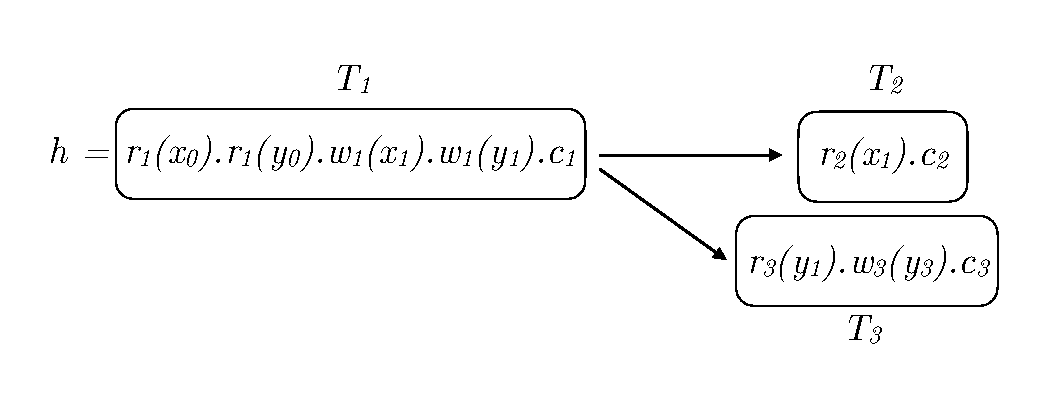
\includegraphics[width=0.7\textwidth]{figures/history.pdf}
  \vspace{-1cm}
  \caption{Example of history represented as a graph. Arrows represent the causal dependencies between operations. Adapted from \em{Saeida Ardekani~\citep{ardekani_thesis}}.}
  \label{fig:history}
\end{figure}

Figure~\ref{fig:history} above shows an example, with $\tx_1 \hb_h \tx_3$ and $\tx_1 \hb_h \tx_2$. We say that two transactions $\tx_i$ and $\tx_j$ are \textbf{\em concurrent} in $h$ (denoted by $\tx_i \parallel \tx_j$) if neither $\tx_i \hb_h \tx_j$ nor $\tx_j \hb_h \tx_j$. In the figure above, $\tx_2$ and $\tx_3$ are concurrent.

\todo{Introduce distributed system here? Or is it covered in chapter 1?}

\section{Consistency Models}

In this section, we define what a consistency model is, distinguishing between \emph{strong} and \emph{weak} models. We give an overview of several models, and compare them in terms of their undesirable effects.

We define a consistency model as a set of histories $\Cons$, such that $\Cons \subseteq \Hist$. Intuitively, a consistency model \emph{constrains} the set of possible histories by specifying how operations interleave in any given history. We say that a given history $h$ \emph{satisfies} a consistency model $\Cons$ if $h \in \Cons$, and that $h$ \emph{violates} $\Cons$.

In the context of databases, the definition of a consistency model maps to the concept of an \emph{isolation level} (I in AC\underline{I}D), which specifies the degree to which concurrent transactions in a database are aware of each other~\citep{adya_thesis}. We use the term consistency throughout this thesis, in accordance with Adya~\citep{adya_thesis}.

Traditionally, the different consistency models have been defined in terms of \emph{anomalies}~\citep{sql-critique}, that map to a set of undesirable histories that are observable by the system. Intuitively, we can distinguish between \emph{strong} and \emph{weak} consistency models depending on the number of anomalies they disallow, with stronger models restricting the set of possible histories more than weak ones. In the sections that follow, we give a brief overview of the traditional anomalies following the definitions advanced by Berenson et al.~\citep{sql-critique}, as well as different consistency models that preclude them. % Figure~\ref{fig:anomalies} shows a quick summary of the models and anomalies we cover.

% \begin{figure}[h]
% \begin{center}
% \begin{tabularx}{\linewidth}{ >{\centering}p{8cm} | *{5}{>{\centering}X}}
%     \multirow{2}{*}{\em Anomalies} & \multicolumn{5}{c}{Consistency Models} \tabularnewline \cline{2-6}
%     & SER & SI & PSI & NMSI & RC \tabularnewline \hline
%     Dirty Write & x & x & x & x & x \tabularnewline
%     Dirty Read & x & x & x & x & x \tabularnewline
%     \hline % Distinguish between ACID or not
%     Non-Repeatable Read & x & x & x & x & \checkmark \tabularnewline
%     Lost Update & x & x & x & x & \checkmark \tabularnewline
%     \hline % Distinguish between weak and strong
%     Write Skew & x & \checkmark & \checkmark & \checkmark & \checkmark \tabularnewline
%     Long Fork & x & x & \checkmark & \checkmark & \checkmark \tabularnewline
% \end{tabularx}
% \end{center}
% \caption{Anomaly Comparison of Consistency Models \emph{(x}:disallowed, \checkmark:allowed\emph{)}. Adapted from \em{Saeida Ardekani et al.~\citep{ardekani-nsmi}}.}
% \label{fig:anomalies}
% \end{figure}

\begin{definition}[Dirty Write]
A \emph{Dirty Write} occurs in a history $h$ when a transaction $\tx_i$ modifies an object $x$ that was previously modified by another pending transaction $\tx_j$. If any of the two transactions commit or abort, it is not clear what value the object $x$ should have. A Dirty Write can be represented by a history such as $w_1(x_1).w_2(x_2).(c_1 \vee a_1).(c_2 \vee a_2)$, where the termination order of the transactions can be arbitrary. The anomaly occurs even if any of the transactions aborts.
\end{definition}

\begin{definition}[Dirty Read]
A \emph{Dirty Read} occurs in a history $h$ when a transaction $\tx_i$ reads an object $x$ modified by a pending transaction $\tx_j$. If $\tx_j$ ultimately aborts in $h$, the value observed by a $\tx_i$ was never supposed to occur in $h$. This is represented by a history such as $r_1(x_0)\ldots w_1(x_1)\ldots r_2(x_1)\ldots c_2\ldots a_1$.
\end{definition}

Both of these anomalies can be prevented by making a transaction's changes visible only after it commits. For example, updates can be buffered locally in the context of a transaction. All the consistency models we describe in the sections that follow preclude dirty writes and reads. Transactions executing under such models offer \emph{atomicity} (A in \underline{A}CID).

\begin{definition}[Non-Repeatable Read]
A non-repeatable read---also called a \emph{fuzzy read}--occurs whenever a transaction $\tx_i$ observes different values for an object $x$ on subsequent read operations when interleaved by a commit by another transaction, $\tx_j$. This can be seen in $r_1(x_0)\ldots r_2(x_0).w_2(x_2).c_2 \ldots r_1(x_2)$. Here, $\tx_1$ observers two different values of $x$: the initial version $x_0$ and the version $x_2$ written by $\tx_2$.
\end{definition}

The non-repeatable read anomaly can also be prevented in an easy way: a transaction can keep a cache of already read values. Subsequent read operations can return values from this read cache.

\begin{definition}[Lost Update]
A \emph{Lost Update} occurs in a history $h$ when two concurrent transactions update the same object $x$ and successfully commit. In this case, the update written by whichever transaction commits first is ``lost'' after the second transaction commits. This can be seen in a history such as $r_1(x_0)\ldots r_2(x_0).w_2(x_2) \ldots w_1(x_1).c_1\ldots c_2$. After $\tx_2$ commits, version $x_1$ is no longer visible to subsequent transactions.
\end{definition}

For the purposes of this thesis, and following the definition used by Saeida Ardekani~\citep{ardekani_thesis}, we say that a consistency model is \emph{strong} if it prevents concurrent transactions to modify the same object. That is to say, a strong consistency model preclude dirty writes and reads, along with lost update anomaly. A model that allows concurrent transactions to modify the same object is \emph{weak}.

We now review several well-known strong consistency models, along with a weak model that will serve as a baseline comparison in the following chapters.

\subsection{Serialisability (SER)}

Serialisability restricts the set of possible histories to those equivalent to some \emph{serial} execution. That is to say, under a traditional system offering Serialisability, the happens-before relation we introduced in~\ref{sect:histories} is strengthened with a \emph{strict total order} over the transactions in a history \todo{does it need to be strict?}. A history such as the one in Figure~\ref{fig:history} is serialisable, because we can order $\tx_2$ to occur before $\tx_3$ (or vice versa); while the one depicted in Figure~\ref{fig:non_ser_history} is not.

\begin{figure}[h]
  \centering
  \vspace{-0.3cm}
  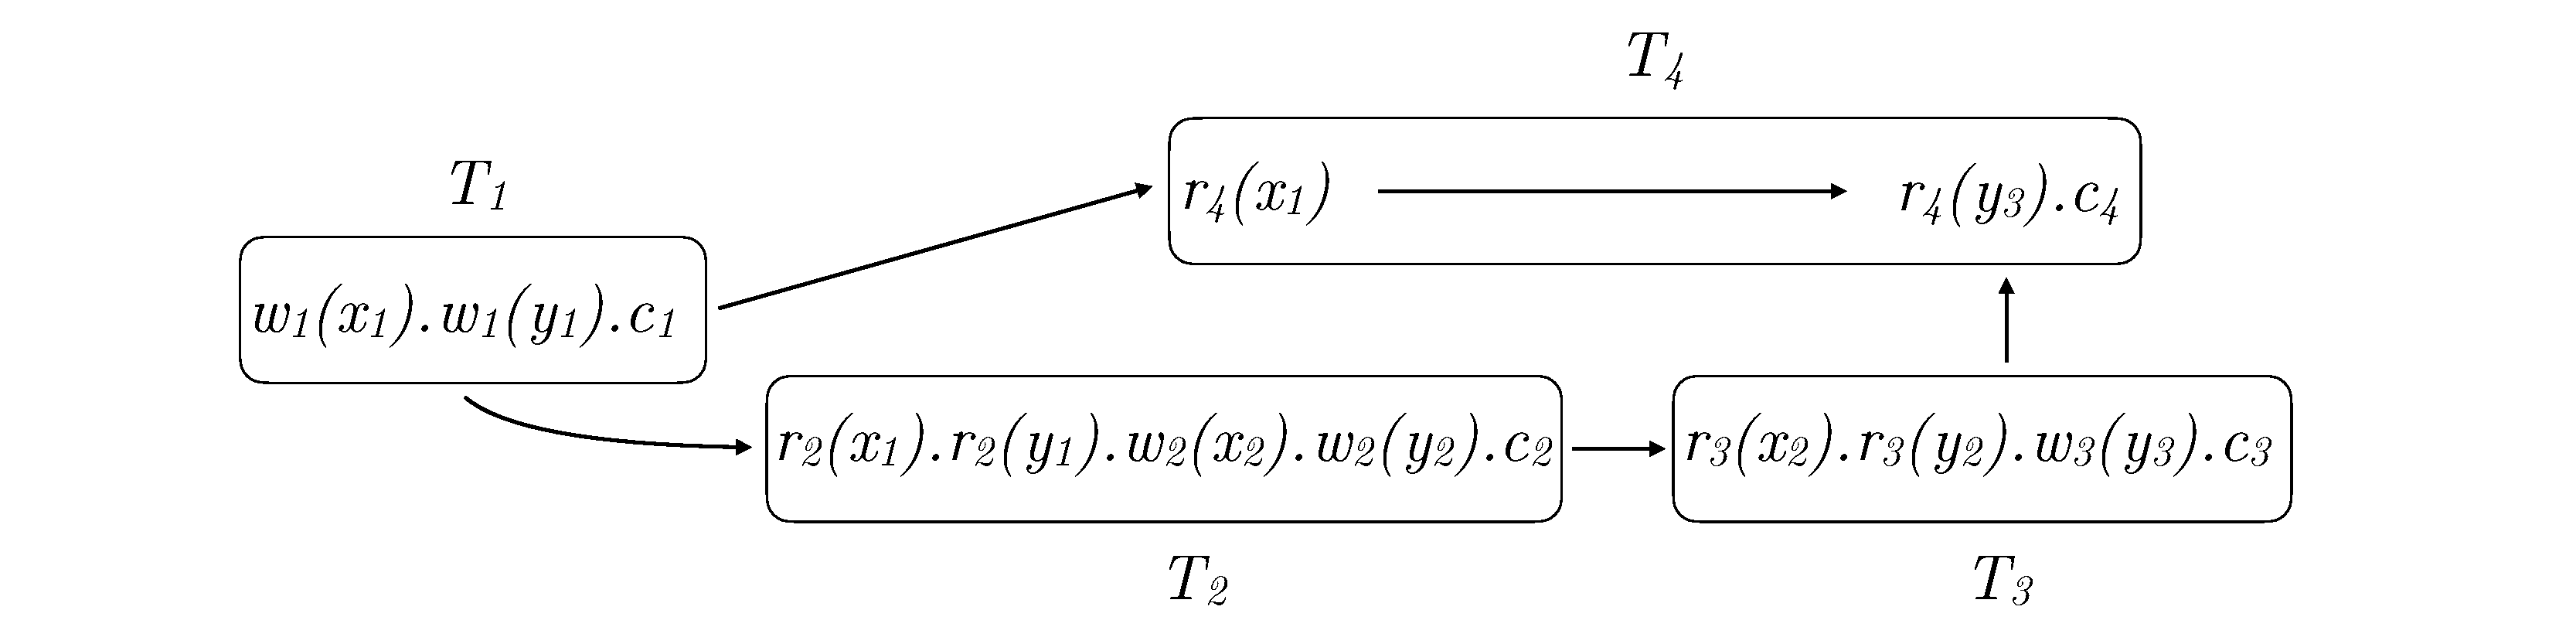
\includegraphics[width=\textwidth]{figures/non_ser_hist.pdf}
  \vspace{-1cm}
  \caption{Example of a non-serialisable history. $\tx_4$ observes version $y_3$ written by $\tx_3$, but fails to observe version $x_2$ written by $\tx_1$. This result can't be obtained by executing the transactions in any sequence, and thus the history is not serialisable.}
  \label{fig:non_ser_history}
\end{figure}

\todo{Mention something about serial order being hard to achieve in a distributed setting?}

\subsection{Snapshot Isolation (SI)}
\label{sect:si}

Proposed by Berenson et al.~\citep{sql-critique}, Snapshot Isolation (SI) relaxes the total ordering guarantees of Serialisability by requiring only a partial order among committed transactions. To preclude the Lost Update anomaly, SI introduces the concept of a \emph{snapshot}: a private view of the data written by committed transactions. This snapshot is created at the time the transaction starts, called its \emph{start timestamp}. A transaction $\tx$ is not able to see updates made by other transactions that commit after $\tx$'s start timestamp. When a transaction $\tx$ is ready to commit, it gets assigned a \emph{commit timestamp}, larger than any previous start or commit timestamp. Transaction $\tx$ commits successfully only if no other concurrent transaction updated the same objects as $\tx$. Under SI, two transactions are concurrent if their start-commit timestamps intervals overlap, and read-only transactions always commit. When two transactions update a non-disjoint set of objects, we say they \textbf{\em write-conflict}.

Due to partial ordering among committed transactions, along with the condition that concurrent transactions only abort if their set of updated objects overlap, a system under Snapshot Isolation is able observe the so-called \emph{Write Skew} anomaly. This anomaly occurs when an external invariant is violated as a result of concurrent non-conflicting transactions. As an example, suppose that objects $x$ and $y$ are related by a constraint such that $x + y \le 10$, with $x = 5$ and $y = 2$ as the initial state. In such a setting, a history such as the following can violate the invariant: $h = r_1(x=5).r_1(y=2).r_2(x=5).r_2(y=2).w_1(x=7).w_2(y=4).c_1.c_2$. Both $\tx_1$ and $\tx_2$ start their execution and observe a consistent state that upholds the invariant. Then, $\tx_1$ updates the object $x$ to the value $7$, which still maintains the invariant, as $7 + 2 \le 10$. Concurrently, $\tx_2$ proceeds as $\tx_1$, updating $y$ to $4$, which also maintains the original invariant ($5 + 4 \le 10$). However, as the result of both $\tx_1$ and $\tx_2$ successfully committing, the invariant is violated, with $7 + 4 \not\le 10$.

%  Figure~\ref{fig:write_skew_history} shows an example of such a history.

% Reads and updates are performed against the transaction snapshot (precluding non-repeatable reads) and made visible after the transaction commits (precluding dirty reads and writes).

% \begin{figure}[h]
%   \centering
%   \vspace{-0.4cm}
%   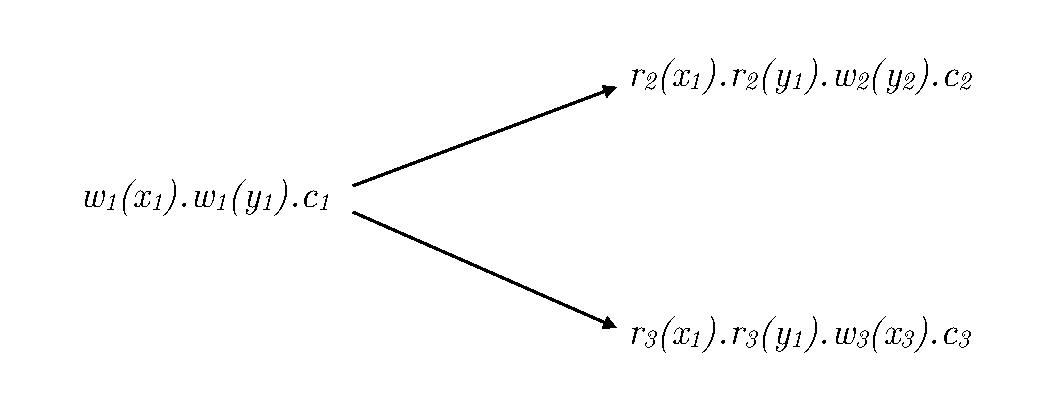
\includegraphics[width=0.6\textwidth]{figures/skew_history.pdf}
%   \vspace{-0.6cm}
%   \caption{Example of a history showing the write skew anomaly. Both $\tx_2$ and $\tx_3$ observe a consistent state of objects $x$ and $y$, but the versions diverge after both transactions commit.}
%   \label{fig:write_skew_history}
% \end{figure}

\begin{definition}[Write Skew]\todo{Revise}
A \emph{Write Skew} occurs whenever two non-conflicting transactions update objects related with an external invariant, successfully commit, and as a result violate the original invariant.
\end{definition}

\todo{Limitations?}

\subsection{Parallel Snapshot Isolation (PSI)}

% From Sovran:
% Snapshot isolation is inadequate for a system replicated at many sites, due to two issues. First, to define snapshots, snapshot isolation imposes a total ordering of the commit time of all transactions, even those that do not conflict. Establishing such an ordering when transactions execute at different sites is inefficient. Second, the writes of a committed transaction must be immediately visible to later transactions. Therefore a transaction can commit only after its writes have been propagated to all remote replicas, thereby precluding asynchronous propagation of its updates.

Parallel Snapshot Isolation (PSI), proposed by Sovran et al.~\citep{psi-intro}, relaxes some of the guarantees offered by classical Snapshot Isolation. Recall from section~\ref{sect:si} that transactions in a system offering SI require monotonically-increasing \emph{start} and \emph{commit} timestamps. The presence of these timestamps require the system to maintain a total order among the commit time of transactions: a so-called total \textbf{\em commit order}. Total order guarantees are challenging to scale in the context of geographically replicated systems, which becomes the principal motivation for the introduction of Parallel Snapshot Isolation. Non-conflicting transactions executing under PSI are allowed to exhibit a relative commit order that varies between replicas. Conflicting transactions are not allowed, as in Snapshot Isolation.

Allowing different commit orderings for non-conflicting transactions at different replicas (or \emph{sites}) makes PSI susceptible to the \emph{Long Fork} anomaly~\citep{psi-intro}. Consider the history depicted in Figure~\ref{fig:long_fork_history}. If transactions $\tx_3$ and $\tx_4$ are executing in different sites, they might observe different commit orderings for $\tx_1$ and $\tx_3$.

\begin{figure}[h]
  \centering
  \vspace{-0.5cm}
  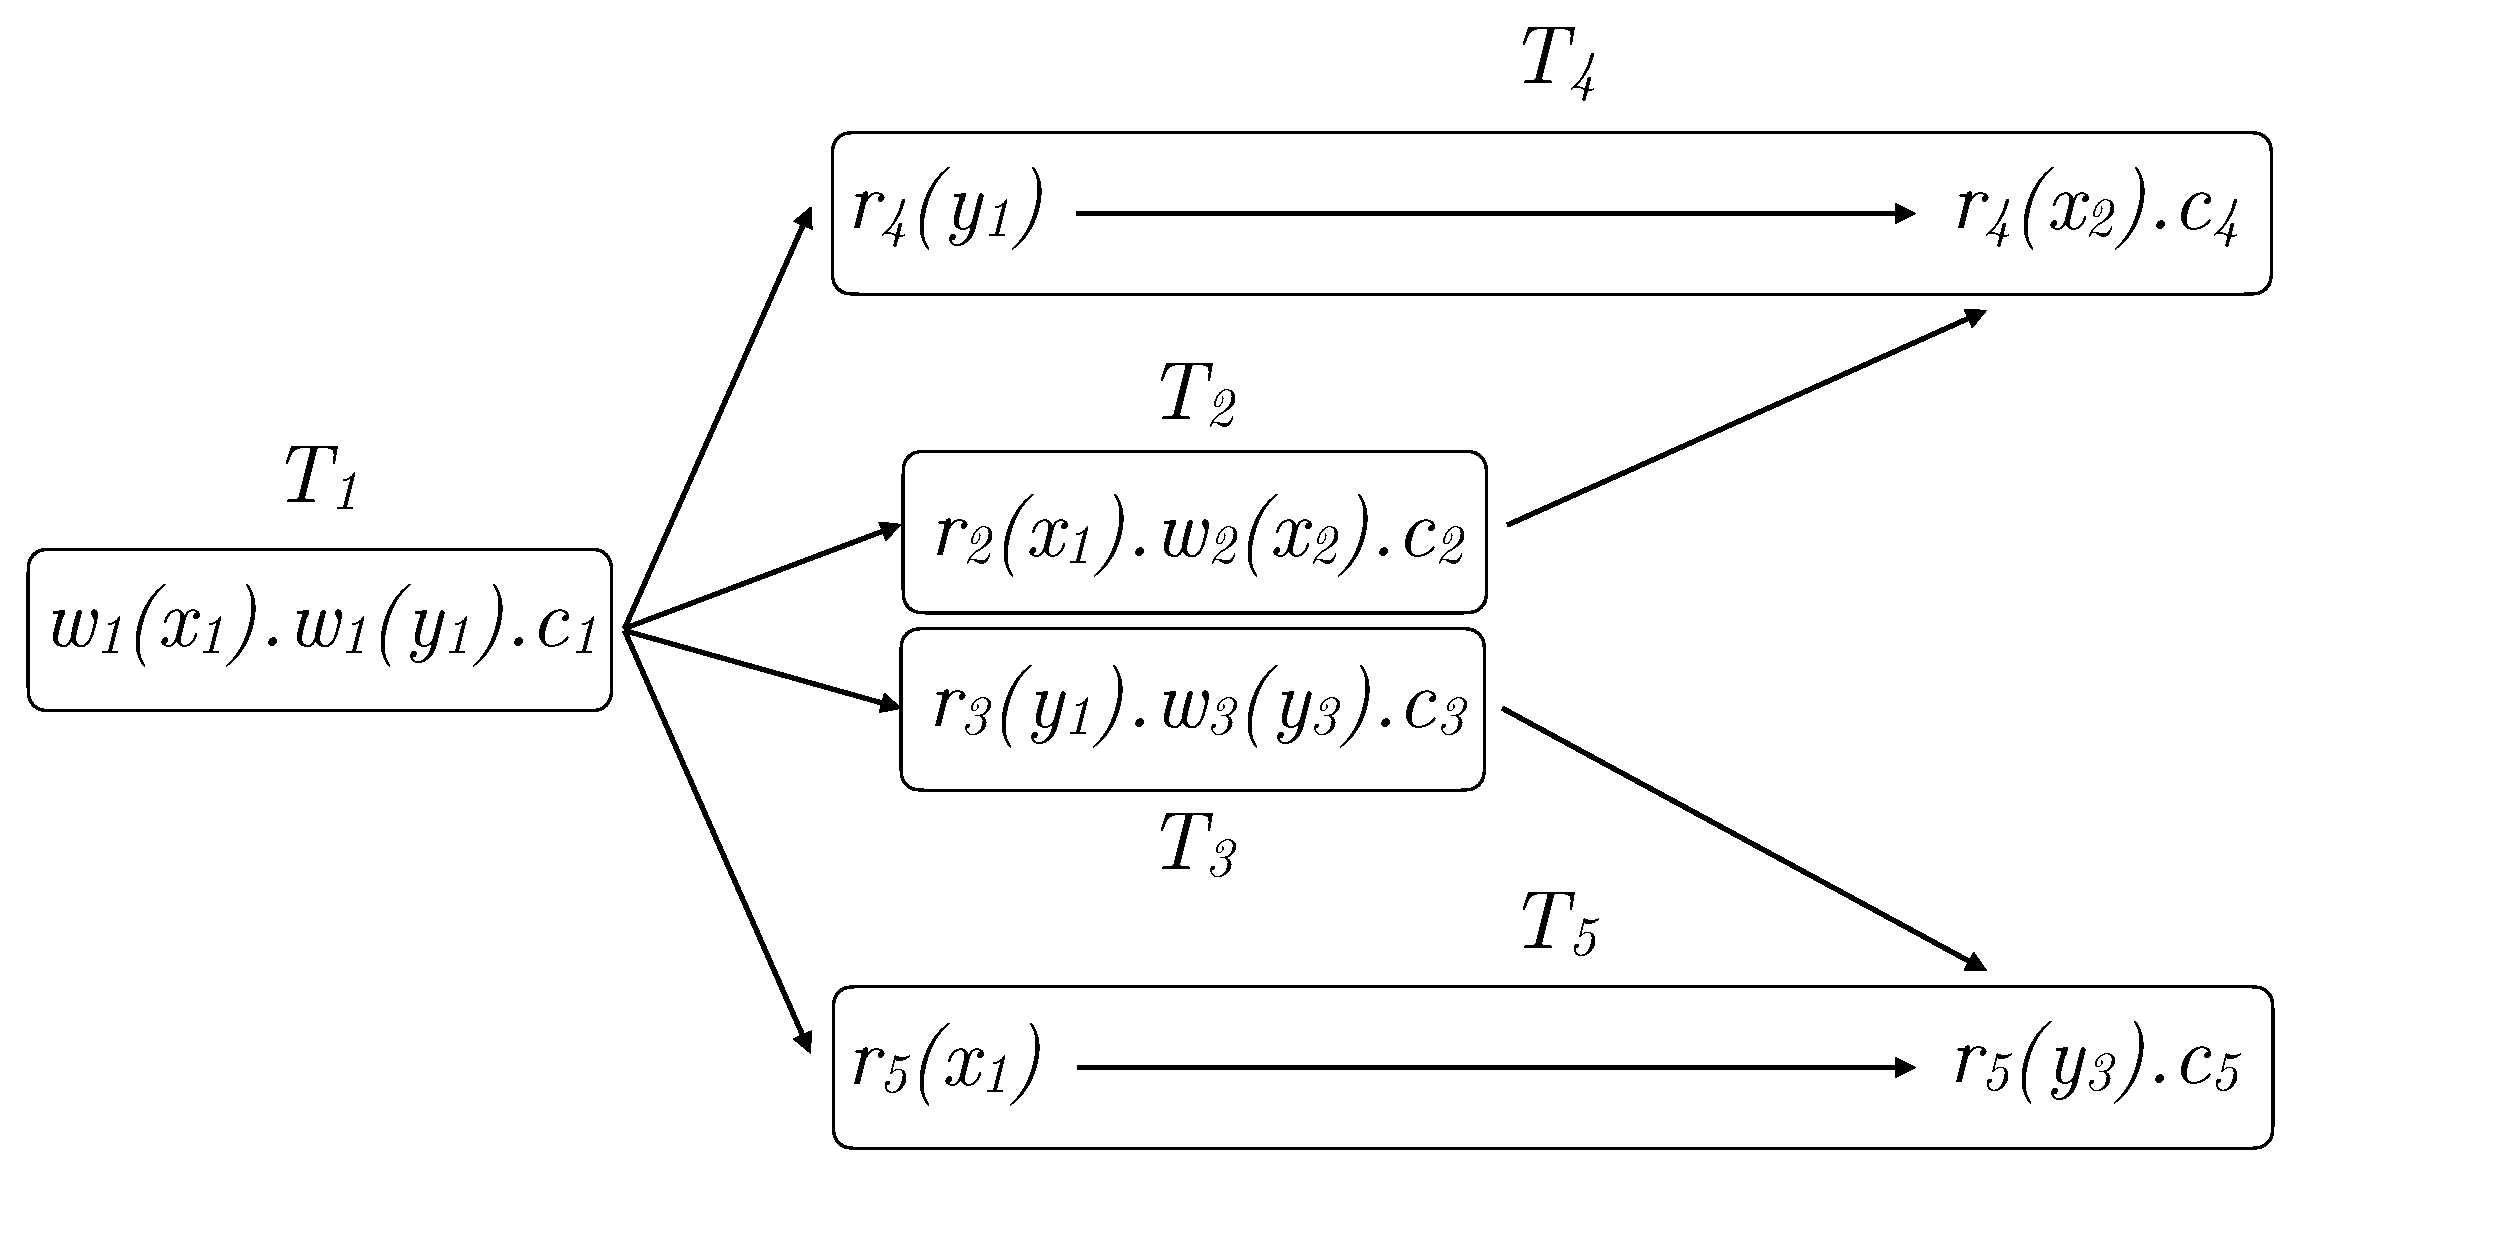
\includegraphics[width=0.7\textwidth]{figures/long_fork_hist.pdf}
  \vspace{-0.5cm}
  \caption{Example of a history showing the long fork anomaly. Transaction $\tx_3$ observes $\tx_1 \rightarrow \tx_2$ while $\tx_4$ observes $\tx_2 \rightarrow \tx_1$. Adapted from \em{Saeida Ardekani~\citep{ardekani_thesis}}.}
  \label{fig:long_fork_history}
\end{figure}

\begin{definition}[Long Fork]
A \emph{Long Fork} occurs whenever a transaction is able to observe different orderings of previous non-conflicting update transactions.
\end{definition}

\todo{Mention causal ordering while replicating?}

\subsection{Non-Monotonic Snapshot Isolation (NMSI)}

\todo{Specification of NMSI (PSI timestamp is fixed at tx.start() time (base freshness), which causes stale transactions in geo-replicated settings.) How big of a deal are anomalies in the applications that we target?}

\todo{From \textit{Making PSI serialisable}: Saeida Ardekani et al. have proposed a variant of PSI called non-monotonic snapshot isolation (NMSI). It is possible to prove that PSI and NMSI produce the same set of anomalies, provided that database clients cannot observe the real-time order between operations: the difference between them lies only in the concurrency control algorithm used. Hence, our results are equally applicable to NMSI.}

\subsection{Read Committed (RC)}

Read Committed is the weakest protocol that satisfies the atomicity guarantee of transactions, by preventing dirty reads and writes. Although this model specifies that all or none of the updates by a transaction are applied to the database, it does not prevent concurrent transactions from observing only a subset of those updates. In this thesis, we use Read Committed as a baseline against which we compare the protocols we implement. \todo{Anything else?}

\subsection{Anomaly Comparison}

Figure~\ref{fig:anomalies} summarises the consistency models we reviewed together with the anomalies that they allow.

\begin{figure}[h]
\begin{center}
\begin{tabularx}{\linewidth}{ >{\centering}p{8cm} | *{5}{>{\centering}X}}
    \multirow{2}{*}{\em Anomalies} & \multicolumn{5}{c}{Consistency Models} \tabularnewline \cline{2-6}
    & SER & SI & PSI & NMSI & RC \tabularnewline \hline
    Dirty Write & x & x & x & x & x \tabularnewline
    Dirty Read & x & x & x & x & x \tabularnewline
    \hline % Distinguish between ACID or not
    Non-Repeatable Read & x & x & x & x & \checkmark \tabularnewline
    Lost Update & x & x & x & x & \checkmark \tabularnewline
    \hline % Distinguish between weak and strong
    Write Skew & x & \checkmark & \checkmark & \checkmark & \checkmark \tabularnewline
    Long Fork & x & x & \checkmark & \checkmark & \checkmark \tabularnewline
\end{tabularx}
\end{center}
\caption{Anomaly Comparison of Consistency Models \emph{(x}:disallowed, \checkmark:allowed\emph{)}. Adapted from \em{Saeida Ardekani et al.~\citep{ardekani-nsmi}}.}
\label{fig:anomalies}
\end{figure}

\section{Catalog of Protocols}
\subsection{Walter}
\subsection{Jessy}
% \subsection{GMU} Tentative, since we don't talk about US in previous section

   \cleardoublepage
\chapter{The fastPSI protocol}
\label{chapter:protocol}

In this chapter we describe \textbf{fastPSI}, a transactional protocol that implements Parallel Snapshot Isolation and allows stronger consistency guarantees for transactions accessing objects inside \emph{entity groups}. We begin with an overview of what entity groups are, and by explaining the consistency guarantees of fastPSI for transactions executing both within and across different groups. We follow with a summary of how the different participants of the protocol interact with each other, and with a description of the different data structures involved. Next, we show how the protocol is structured by going over the execution of a transaction. We conclude with a discussion of the possible drawbacks of the design.

\section{Consistency Guarantees}

The fastPSI protocol considers a system in which objects are aggregated in \emph{entity groups}~\citep{baker_megastore}. An entity group $\sigma$ is defined as a proper partition of objects $\Obj$. This means that two properties hold: (i) $\forall \sigma, \sigma' \implies \sigma \cap \sigma' = \emptyset$, and (ii) $\forall x \in \Obj .\ \exists \sigma .\ x \in \sigma$. The first property says that the sets of objects covered by different entity groups are \emph{disjoint}, while the second property states that any object that exists in the system is part of an entity group.

The goal of fastPSI is as follows: transactions that only access objects inside a single entity group should satisfy Snapshot Isolation (SI), while transactions that access objects across entity groups should satisfy Parallel Snapshot Isolation (PSI). Intuitively, if one has a single entity group that encompasses every object, any execution of fastPSI is equivalent to an execution under Snapshot Isolation, thereby precluding the Long Fork anomaly. Conversely, if one has an entity group per object in the system, then any execution of fastPSI is equivalent to an execution under Parallel Snapshot Isolation. The decision of which objects to place into different entity groups is left to the programmer, who should take application requirements into account.

Recall from Section~\ref{sect:si} that transactions executing under SI are only partially ordered, in contrast with serialisability, where they are totally ordered. However, the requirement for transactions to take monotonic \emph{start} and \emph{commit} timestamps induces a total \emph{commit order} for transactions, even for those that are not in conflict with each other. In the presence of different entity groups, this requirement would require transactions to communicate with every group in order to determine a monotonic timestamp. In fastPSI, we relax this requirement so that transactions have multiple, independent timestamps, one per entity group.

In order to guarantee Parallel Snapshot Isolation across entity groups, we incorporate the notion of forward freshness~\citep{ardekani_nmsi}, which allows a transaction $\tx$ to read versions of objects written by transactions that committed after $\tx$ starts. The fastPSI protocol accomplishes this by making a transaction $\tx$ fix its start timestamp at a particular entity group only when $\tx$ reads an object from that group. This also allows a transaction to acquire start timestamps only at the groups it reads from, thus avoiding coordination with other groups.

The fastPSI protocol leverages both approaches to offer its consistency guarantees: a transaction is able to read from versions written by latter transactions as long as those reads form a \emph{causally consistent snapshot}. When a transaction $\tx$ performs its first read operation in an entity group, it fixes a snapshot that includes all the transactions that committed before $\tx$'s read occurred. As $\tx$ performs further read operations on other entity groups, the snapshots that $\tx$ fixes are restricted to versions written by transactions that are not causally dependent on the transactions that $\tx$ already included in its previous snapshots.

\section{Overview and System Model}
\label{sect:protocol_overview}

The protocol consists of three components: \emph{client} processes that provide the system interface for managing transactions, \emph{server} processes that handle the individual operations of transactions, and \emph{entity groups}---managed by a server---which store individual data objects. Given that entity groups properly divide the range of objects into disjoint \emph{partitions}, for the remainder of this chapter we use the term partition as a shorthand for entity group.

Both client and server processes are considered reliable and connected by reliable channels\footnote{Fault-tolerance concerns are orthogonal to the problem we address, although several approaches are discussed in Chapter~\ref{chapter:related_work}.}. Processes communicate with each other using an asynchronous message-passing system. We denote the server processes as a set $\mathcal{S} = \{s_1, \dots, s_N\}$, and clients as $\mathcal{C} = \{c_1, \dots, c_M\}$. Data objects are denoted by a set $\Obj$, split into $N$ partitions, each stored by a server process. We let $\partitionOf(x)$ be the index of the partition the object $x$ belongs to, such that it is managed by server $s_{\partitionOf(x)}$. For simplicity, we assume that server processes only manage a single partition.

\emph{Clients} provide the transactional interface of the protocol through the \texttt{start}, \texttt{read}, \texttt{write} and \texttt{commit} operations. Transactions are \emph{interactive}, i.e., when a transaction starts, the client does not know which operations it will perform in advance. In fastPSI, the \texttt{start} and \texttt{write} operations are local to the client. Clients issue \texttt{read} operations to servers, which return the values and metadata associated with the objects the client requested. Clients handle \texttt{write} operations locally by storing the updates in a buffer, called the \emph{write-set} of a transaction. At \texttt{commit} time, the client acts a coordinator of a \emph{two-phase commit protocol (2PC)}~\citep{bernstein_concurrency}, issuing \texttt{prepare} and \texttt{decide} operations to all the participating servers. The written values buffered locally are transmitted to the servers at \texttt{prepare} time, together with the accumulated metadata for the objects that the client read. The decision to commit or abort a transaction is taken based on this metadata.

\emph{Servers} handle three operations issued by clients: \texttt{read}, \texttt{prepare} and \texttt{decide}. When a server handles \texttt{read} operations, it forwards the request to the partition responsible for the object being requested. When receiving a \texttt{prepare} request for a certain transaction, the server checks for conflicts with other transactions waiting to be decided, which are stored in a commit queue. If the transaction contained in the client request does not conflict, it is added to the queue, and the server replies to the client with a $\commit$ vote. If, on the other hand, the transaction is found to be conflicting, an $\abort$ vote is sent instead.

\emph{Partitions} are responsible for fulfilling read requests on behalf of servers, and for maintaining causally consistent snapshots on behalf of the clients. Partitions store multiple \emph{versions} of an object in accordance with a multi-version concurrency control protocol. When executing a read request for an object $x$, a partition finds and returns the most recent causally consistent version of $x$, along with some metadata of the chosen version.

Each partition stores multiple versions of an object represented by a tuple $\langle val, vid \rangle$, where $val$ is the value of a given version, and $vid$ is a logical identifier for the transaction that committed this version. To represent this logical identifier we use \emph{version vectors}~\citep{version-vectors}. Such a vector consists of $N$ entries, one for each partition, storing a non-negative integer. Each entry $vid[i]$ in the vector can also be represented by a pair $(s_i, k)$, where $k$ is the actual value of the $i$-th entry of the vector. We call these pairs a dot~\citep{carlos-causality}. Version vectors are compared according to the following relation, showing when one vector covers more dots than another: $V_1 \sqsubseteq V_2 \iff \forall i.\ V_1[i] \le V_2[i]$. In addition, there exists a \emph{join} operation on vectors, taking their entry-wise maximum, which we will also denote by \emph{max} from now on. We denote the set of all version vectors by $\VCSet$, and the vector with all entries set to $0$ by $\vec{0}$.

\section{Server data structures}
\label{sect:protocol_structures}

\begin{figure}[t]
\noindent\adjustbox{max width=\paperwidth}{\footnotesize
\begin{tabularx}{\linewidth}{|c|p{5.5cm}|X|}
  \hline
  \multicolumn{3}{|c|}{\textbf{Data Structures at a server $s_i$}}\\
  \hline
  $\lastprep$ & {\sf Integer} & The number of update transactions that tried to
  commit at the server.
\\
  \hline
  $\VersionLog$ & ${\sf Map}[\keytype,$ ${\sf
    Set}[\langle \valuetype\ \val, \vctype\ \Vcomm\rangle]]$ & Database:
  a mapping from objects to lists of pairs of a value and the
  commit vector of the transaction that wrote it. The lists are ordered
  by the $i$-th component of the commit vectors.
\\
  \hline
  $\CommitLog$
  & ${\sf Sequence}[\langle\transtype\ T,$ $\vctype\ \Vaggr \rangle]$
  & Log of update transactions $T$ committed at the server, ordered by
  $\Vaggr[i]$. Here $\Vaggr$ is the aggregate vector of $T$: the join of the
  commit vectors of all transactions up to $T$ in $\CommitLog$.
\\
  \hline
  $\LocalTime$ & $\vctype$ & The join of the commit vectors of all
  transactions in $\CommitLog$.
\\
  \hline
  $\CommitQueue$ & ${\sf Sequence}[\langle \transtype, \pending, {\sf WriteSet} \rangle \cup
  \langle \transtype, \ready, {\sf WriteSet}, \vctype\rangle]$ &
  Queue containing information about update transactions trying to commit
  at the server.
\\
  \hline
\end{tabularx}
}
\caption{
  Data structures used by servers in the protocol. The orders of entries in $\CommitLog$, $\VersionLog$ and $\CommitQueue$ are consistent with the commit order of the associated transactions. We select the components of various tuples using the names given in the figure.}
\label{fig:server-structures}
\end{figure}

Each server $s_i$ maintains five main data structures, summarised in Figure~\ref{fig:server-structures}. We now offer a more detailed explanation of each of them.

$\lastprep$ is a counter of the number of update transactions that initiated their commit phase at a given server. When a transaction commits at a server $s_i$, it gets assigned the value of the counter as a \emph{sequence number} $k$, which induces the \emph{commit order} of transactions at $s_i$. A transaction computes its \emph{commit vector} $V_c$ from these sequence numbers, such that the vector represents the set of dots $\{(s_i, k) \mid k \le V_c[i]\}$ which identifies the writes by previous transactions whose sequence number at a server $s_i$ is no higher than $V_c[i]$.

$\VersionLog$ is a mapping of objects to a list of versions, which we call the \emph{database}. As noted before, each version is a tuple $\langle \mathsf{val},\ \Vcomm \rangle$ such that $\mathsf{val}$ is a value and $\Vcomm$ is the commit vector of the transaction that wrote $\mathsf{val}$. The $\VersionLog$ at $s_i$ is ordered by the $i$-th component of the commit vector of each version, which follows the commit order of transactions at the server. We denote by $\VersionLog[x].\last$ the most recent entry in the list for the object $x$.

$\CommitLog$ is an ordered list that maintains a tuple $\langle T,\ \Vaggr \rangle$ for each update transaction that committed at a server, such that $\tx$ is the identifier of a committed transaction and $\Vaggr$ is an \emph{aggregate vector}. The aggregate vector represents the join of the commit vectors of all the transactions up to $\tx$ in $\CommitLog$. Entries in the log at $s_i$ are totally ordered according to the $i$-th entry of their aggregate vectors, $\Vaggr[i]$, which also follows the commit order of transactions at the server. These aggregate vectors are stored for efficiency, and are used to compute the snapshot of a transaction at the server. The aggregate vector of the last committed transaction is stored in $\LocalTime$. Initially, the $\CommitLog$ contains a single placeholder entry $\langle \_, \vec{0} \rangle$.

Finally, $\CommitQueue$ is an ordered queue of transactions trying to commit updates at the server. The queue has entries of two types. An entry $\langle \tx, \pending, \localWS \rangle$ means that $\tx$ is successfully prepared to commit at $s_i$, but the final decision on it is not yet known; $\localWS$ is the \emph{write-set} of the transaction, containing object-value pairs. An entry $\langle \tx, \ready, \localWS, V \rangle$ in the queue means that $\tx$ has been decided to commit with a commit vector $V$, but its writes have not yet been added to the $\VersionLog$. The order of transactions in $\CommitQueue$ follows the commit order at the server.

\section{Protocol Description}

The protocol is now described in detail by following the execution of a transaction. We begin by describing how a transaction is initialised, along with the mechanism to build a causally consistent snapshot. Later, we show the mechanism to validate and commit a transaction.

\subsection{Transaction Execution}
\label{subsect:protocol_execution}

The fastPSI protocol uses optimistic concurrency control, that is, the execution of a transaction is speculative. Clients read objects from servers and buffer writes locally. At the end of the execution, the decision whether to commit or abort a transaction is taken based on the existence of conflicts with concurrently executing transactions. Clients executing a transaction maintain a transaction \emph{context} including several pieces of data, summarised in Figure~\ref{fig:context-variables} and explained below.

In the following, we refer to the algorithms in Figures~\ref{fig:client-init-write} and~\ref{fig:read-local-remote} to describe the steps taken by both clients and servers to execute $\tx$.

\begin{figure}[h]
\noindent\adjustbox{max width=\paperwidth}{\footnotesize
\begin{tabularx}{\linewidth}{|c|p{4cm}|X|}
  \hline
  \multicolumn{3}{|c|}{\textbf{Context for a transaction $T$ at a client $c_i$}} \\
  \hline
  $T.\WS$ & ${\sf WriteSet}$ & Write-set of $T$.
\\
  \hline
  $T.\hasRead$ & ${\sf Vector}[{\sf Bool}]$ & Mapping showing whether $T$  has
  read a given partition.
\\
  \hline
  $T.\VCaggr$ & $\vctype$ & Snapshot vector: determines snapshots fixed at
  partitions $T$ has read from and possible causal dependencies at all other
  partitions.
\\
  \hline
  $T.\VCdep$ & $\vctype$ & Dependency vector, representing all causal
  dependencies developed by $T$ during its execution.
\\
  \hline
\end{tabularx}
}
\caption{
  Data structures used in the transaction context, kept by the clients in the protocol. In the table, ${\sf WriteSet} = {\sf Set}[\langle \keytype, \valuetype \rangle]$
}
\label{fig:context-variables}
\end{figure}

When a client starts a transaction $\tx$, it first initialises its context (line~\ref{alg:start_tx_start}). When a transaction $\tx$ writes a value $v$ to an object $x$ (line~\ref{alg:write_start}), the client buffers this write in $\tx$'s \emph{write-set}, $\tx.\WS$, while discarding any previously written value of $x$.

\begin{figure}[h]
\begin{algorithm}[H]
  \setcounter{AlgoLine}{0}
  % Start
  \SubAlgo{\Fun ${\tt start}()$\label{alg:start_tx_start}}{
    \Return{$\KwSty{new}\ \transtype(\WS= \emptyset, \hasRead =
      \vec{\bot}, \VCaggr = \vec{0}, \VCdep =
      \vec{0})$};\label{alg:start_tx_end}}

  \smallskip

  % Write
  \SubAlgo{\Fun ${\tt write}(T, x, v)$\label{alg:write_start}}{
    $\tx.\WS \leftarrow \left(\tx.\WS\ \backslash\ \{\langle x, \_ \rangle\}\right) \cup \{\langle x,v\rangle\}$\;\label{alg:write_end}
  }
\end{algorithm}
\caption{
  Initialisation of a transaction and update of an object \emph{x} at client $c_i$.
}
\label{fig:client-init-write}
\end{figure}

When the transaction $\tx$ issues a read operation on an object $x$ (line~\ref{alg:read_start}), the client first checks $\tx.\WS$ (line~\ref{alg:read_ws_check}): if $\tx$ has already written to $x$, the value stored in the write-set is returned. Otherwise, and assuming that $j = \partitionOf(x)$, the client sends a $\READREQUEST$ message to the server $s_j$ to fetch the value of the object (line~\ref{alg:read_send}).

When the transaction $\tx$ reads an object from a partition $j$ for the first time, the server $s_j$ fixes a \emph{snapshot} of versions from which it will serve all future reads by $\tx$. This snapshot is defined by an integer $k$: it will include the versions written by all the transactions that committed at the server with a sequence number up to $k$. The client keeps this information in the transaction context, by storing $k$ in the $j$-th entry of a \emph{snapshot vector} $\tx.\VCaggr$, and by marking the current partition as read in $\tx.\hasRead$, a boolean mapping its $j$-th entry to $\top$ if $\tx$ read an object from $s_j$, and $\bot$ otherwise. If $\tx.\hasRead[j]=\top$, then the vector $\tx.\VCaggr$ is equal to the join of the commit vectors of all transactions committed at $s_j$ with a sequence number no higher than $\VCaggr[j]$.

\begin{figure}[h]
\begin{algorithm}[H]
  % Read
  \SubAlgo{\Fun ${\tt read}(T, x)$\label{alg:read_start}}{
    \If{$\langle x, v \rangle \in \tx.\WS$\label{alg:read_ws_check}}{
      \Return{$v$}\;
    }

    $j \leftarrow \partitionof(x)$\;
    \Send{$\READREQUEST(x, T.\VCaggr, T.\hasRead)$} \KwTo $s_j$\;\label{alg:read_send}
    \Receive{$\READRETURN(m)$} \KwFrom $s_j$\;\label{alg:read_recv}
    \uIf{$m = \abort$} {
      \Throw{$\abort$}\;\label{alg:read_abort}
    }
    \ElseIf{$m = \langle v,\localVdep,\localVaggr \rangle$\label{alg:read_msg_decomp}}{
      $\tx.\hasRead[j] \leftarrow \true$\;
      $\tx.\VCdep \leftarrow \max(\tx.\VCdep,\localVdep)$\;\label{alg:read_upd_vcdep}
      $\tx.\VCaggr \leftarrow \max(\tx.\VCaggr,\localVaggr)$\;\label{alg:read_upd_vcaggr}
      \Return{$v$}\;\label{alg:read_end}
    }
  }

  \smallskip

  % ReadRequest
  \SubAlgo{\WhenReceived $\READREQUEST(x, \argVCaggr, \argHasRead)$ \KwFrom $c_j$\label{alg:read_req_start}}{
    \uIf{$\argHasRead[i]$\label{alg:read_req_read_check}} {
      $V \leftarrow \argVCaggr$\;\label{alg:read_req_read_maxvc}
    }
    \Else{\label{alg:read_req_read_check_else}
      \Until{$\mrvc[i] \ge \argVCaggr[i]$}\;\label{alg:read_req_wait}
      $r \leftarrow \max\{r \in \CommitLog \mid \forall j.\, \argHasRead[j] {\implies} \left(r.\Vaggr[j] \le \argVCaggr[j]\right)\}$\;\label{alg:max_vc_search}
      \If{$r.\Vaggr[i] < \argVCaggr[i]$\label{alg:read_req_abort_check}}{
        \Send{$\READRETURN(\abort)$} \KwTo $c_j$\;\label{alg:read_req_abort}
        \Return\;
      }
      $V \leftarrow r.\Vaggr$\;\label{alg:read_req_unread_maxvc}
    }
    $\ver = \max\{\ver \in \VersionLog \mid ver.\Vcomm[i] \le V[i]\}$\; \label{alg:chose-version}
    \Send{$\READRETURN(\ver.\val, \ver.\Vcomm,V)$} \KwTo $c_j$\;\label{alg:read_req_end}
  }
\end{algorithm}
\caption{Local and remote read of object \emph{x}.}
\label{fig:read-local-remote}
\end{figure}

Thus, the entries in the snapshot vector for partitions that $\tx$ has not yet read from delimit all the possible causal dependencies $\tx$ may develop at these partitions.

Both $\tx.\VCaggr$ and $\tx.\hasRead$ are supplied by the client when issuing a read operation on object $x$, by using them as parameters to the $\READREQUEST$ message sent to a server $s_i$. When the server receives this message (line~\ref{alg:read_req_start}), it first checks, using the $\hasRead$ mapping, if the transaction has read from it before (line~\ref{alg:read_req_read_check}). In this case, the snapshot is determined by $\VCaggr[i]$, and the server returns the latest version $\mathit{ver}$ of the object $x$ written by a transaction in the snapshot, i.e., with a sequence number no higher than $\VCaggr[i]$ (line~\ref{alg:chose-version}). This version is determined by examining the $i$-th entry of the commit vectors in $\VersionLog$. The server then replies to the client with a $\READRETURN$ message containing the value of the chosen version and its associated version vector, as well as the unmodified snapshot vector provided by the client: since the server used a previously fixed snapshot, no updates to the vector are required.

% \begin{figure}[t]
% 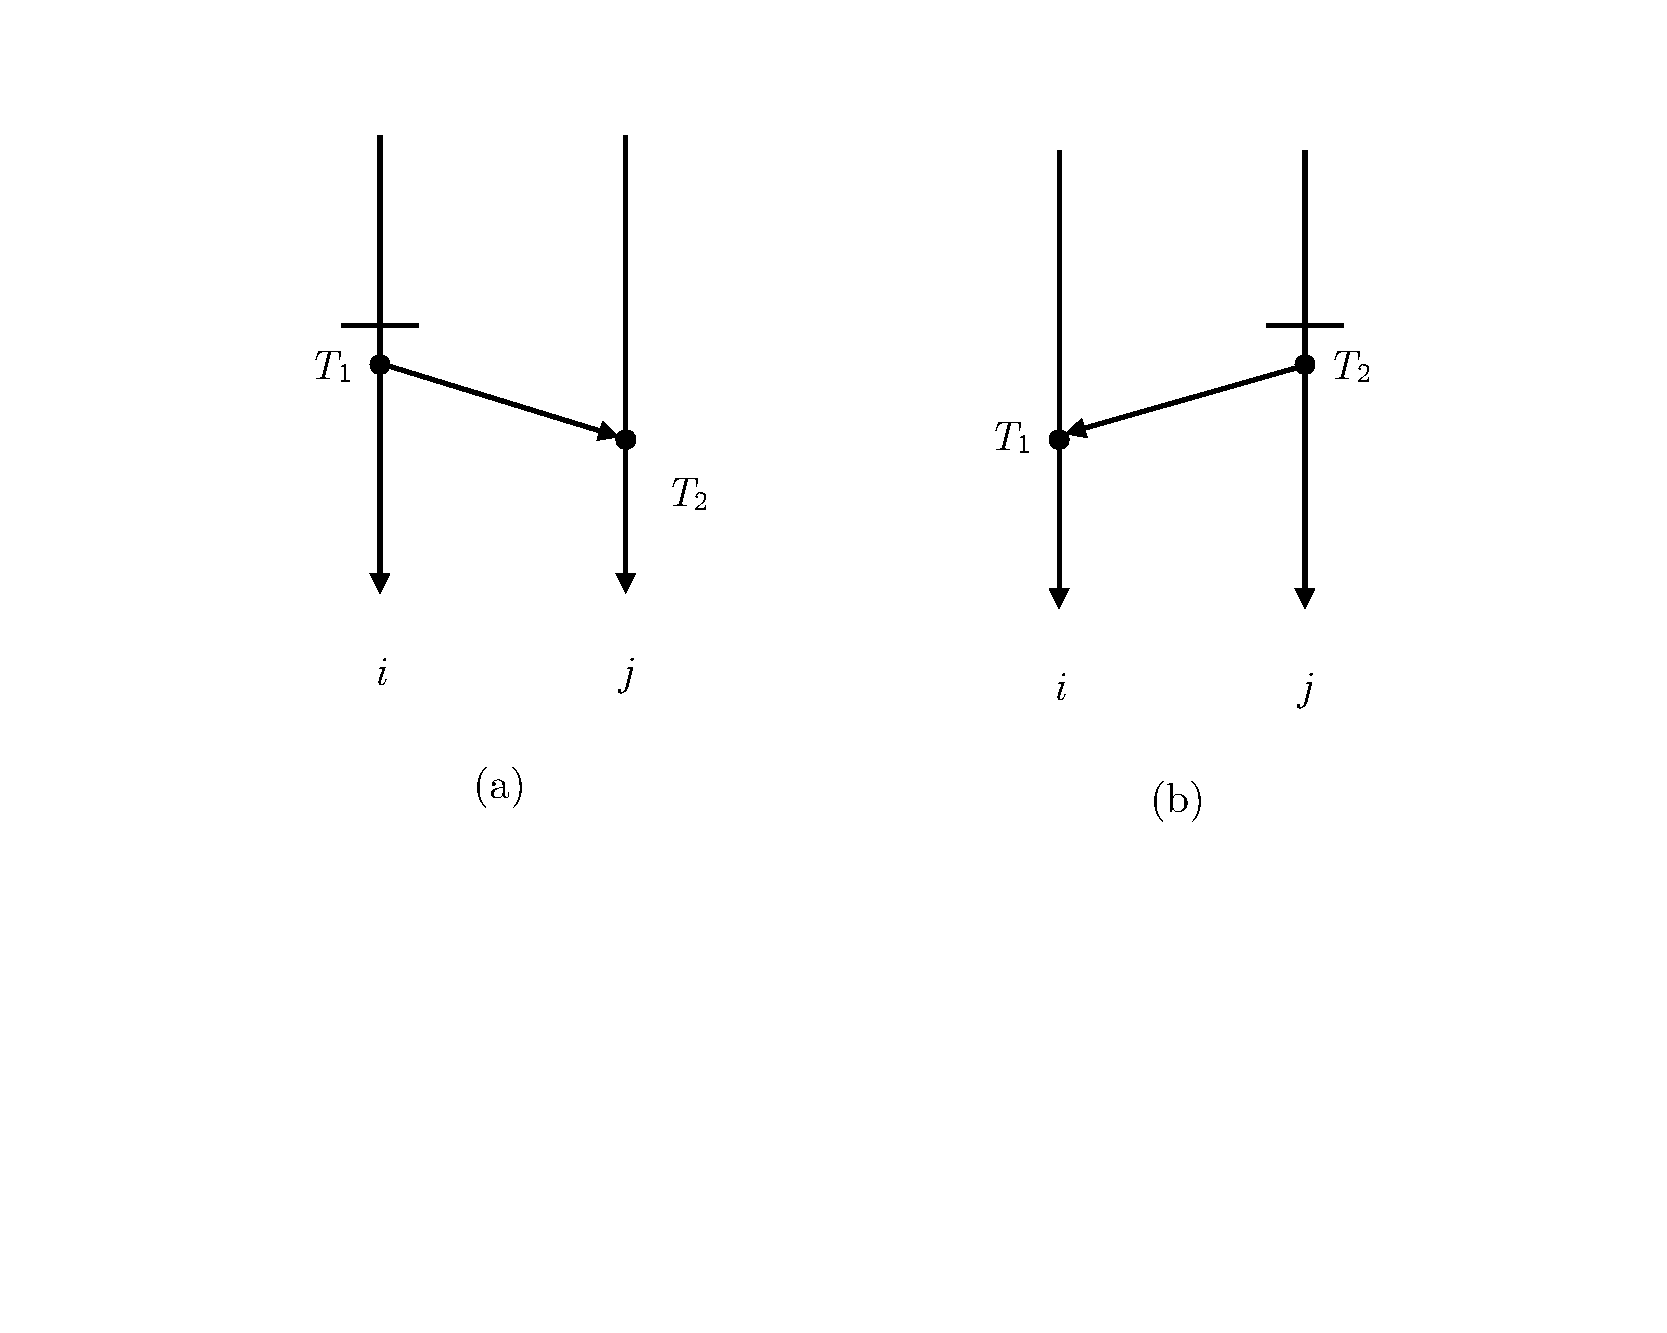
\includegraphics[width=\textwidth]{figures/ch4_snapshot_fork.pdf}
% \vspace{-5.5cm}
% \caption{Illustrations of the snapshot computation. Vertical lines depict the
%   commit order at the corresponding partitions (top to bottom) and horizontal
%   lines the cut-offs of various snapshots. Arrows between partitions depict
%   causal dependencies.}
% \label{fig:fig:snapshot_fork}
% \end{figure}

We now consider the case when the client is reading from the server $s_i$ for the first time (line~\ref{alg:read_req_read_check_else}). In this case, we have to fix the snapshot for the transaction $\tx$ at this server. Choosing a suitable snapshot is complicated by the fact that we allow transactions to be interactive---that is, we do not know in advance which objects a transaction will read in the future. We hence fix the snapshot in such a way that \emph{any} later read from this snapshot will be \emph{causally consistent} with any other read from the snapshots that $\tx$ has already fixed, as specified by $\hasRead$ and $\VCaggr$. To ensure this, the snapshot we select has to satisfy two requirements.

\begin{figure}[t]
\vspace{-0.5cm}
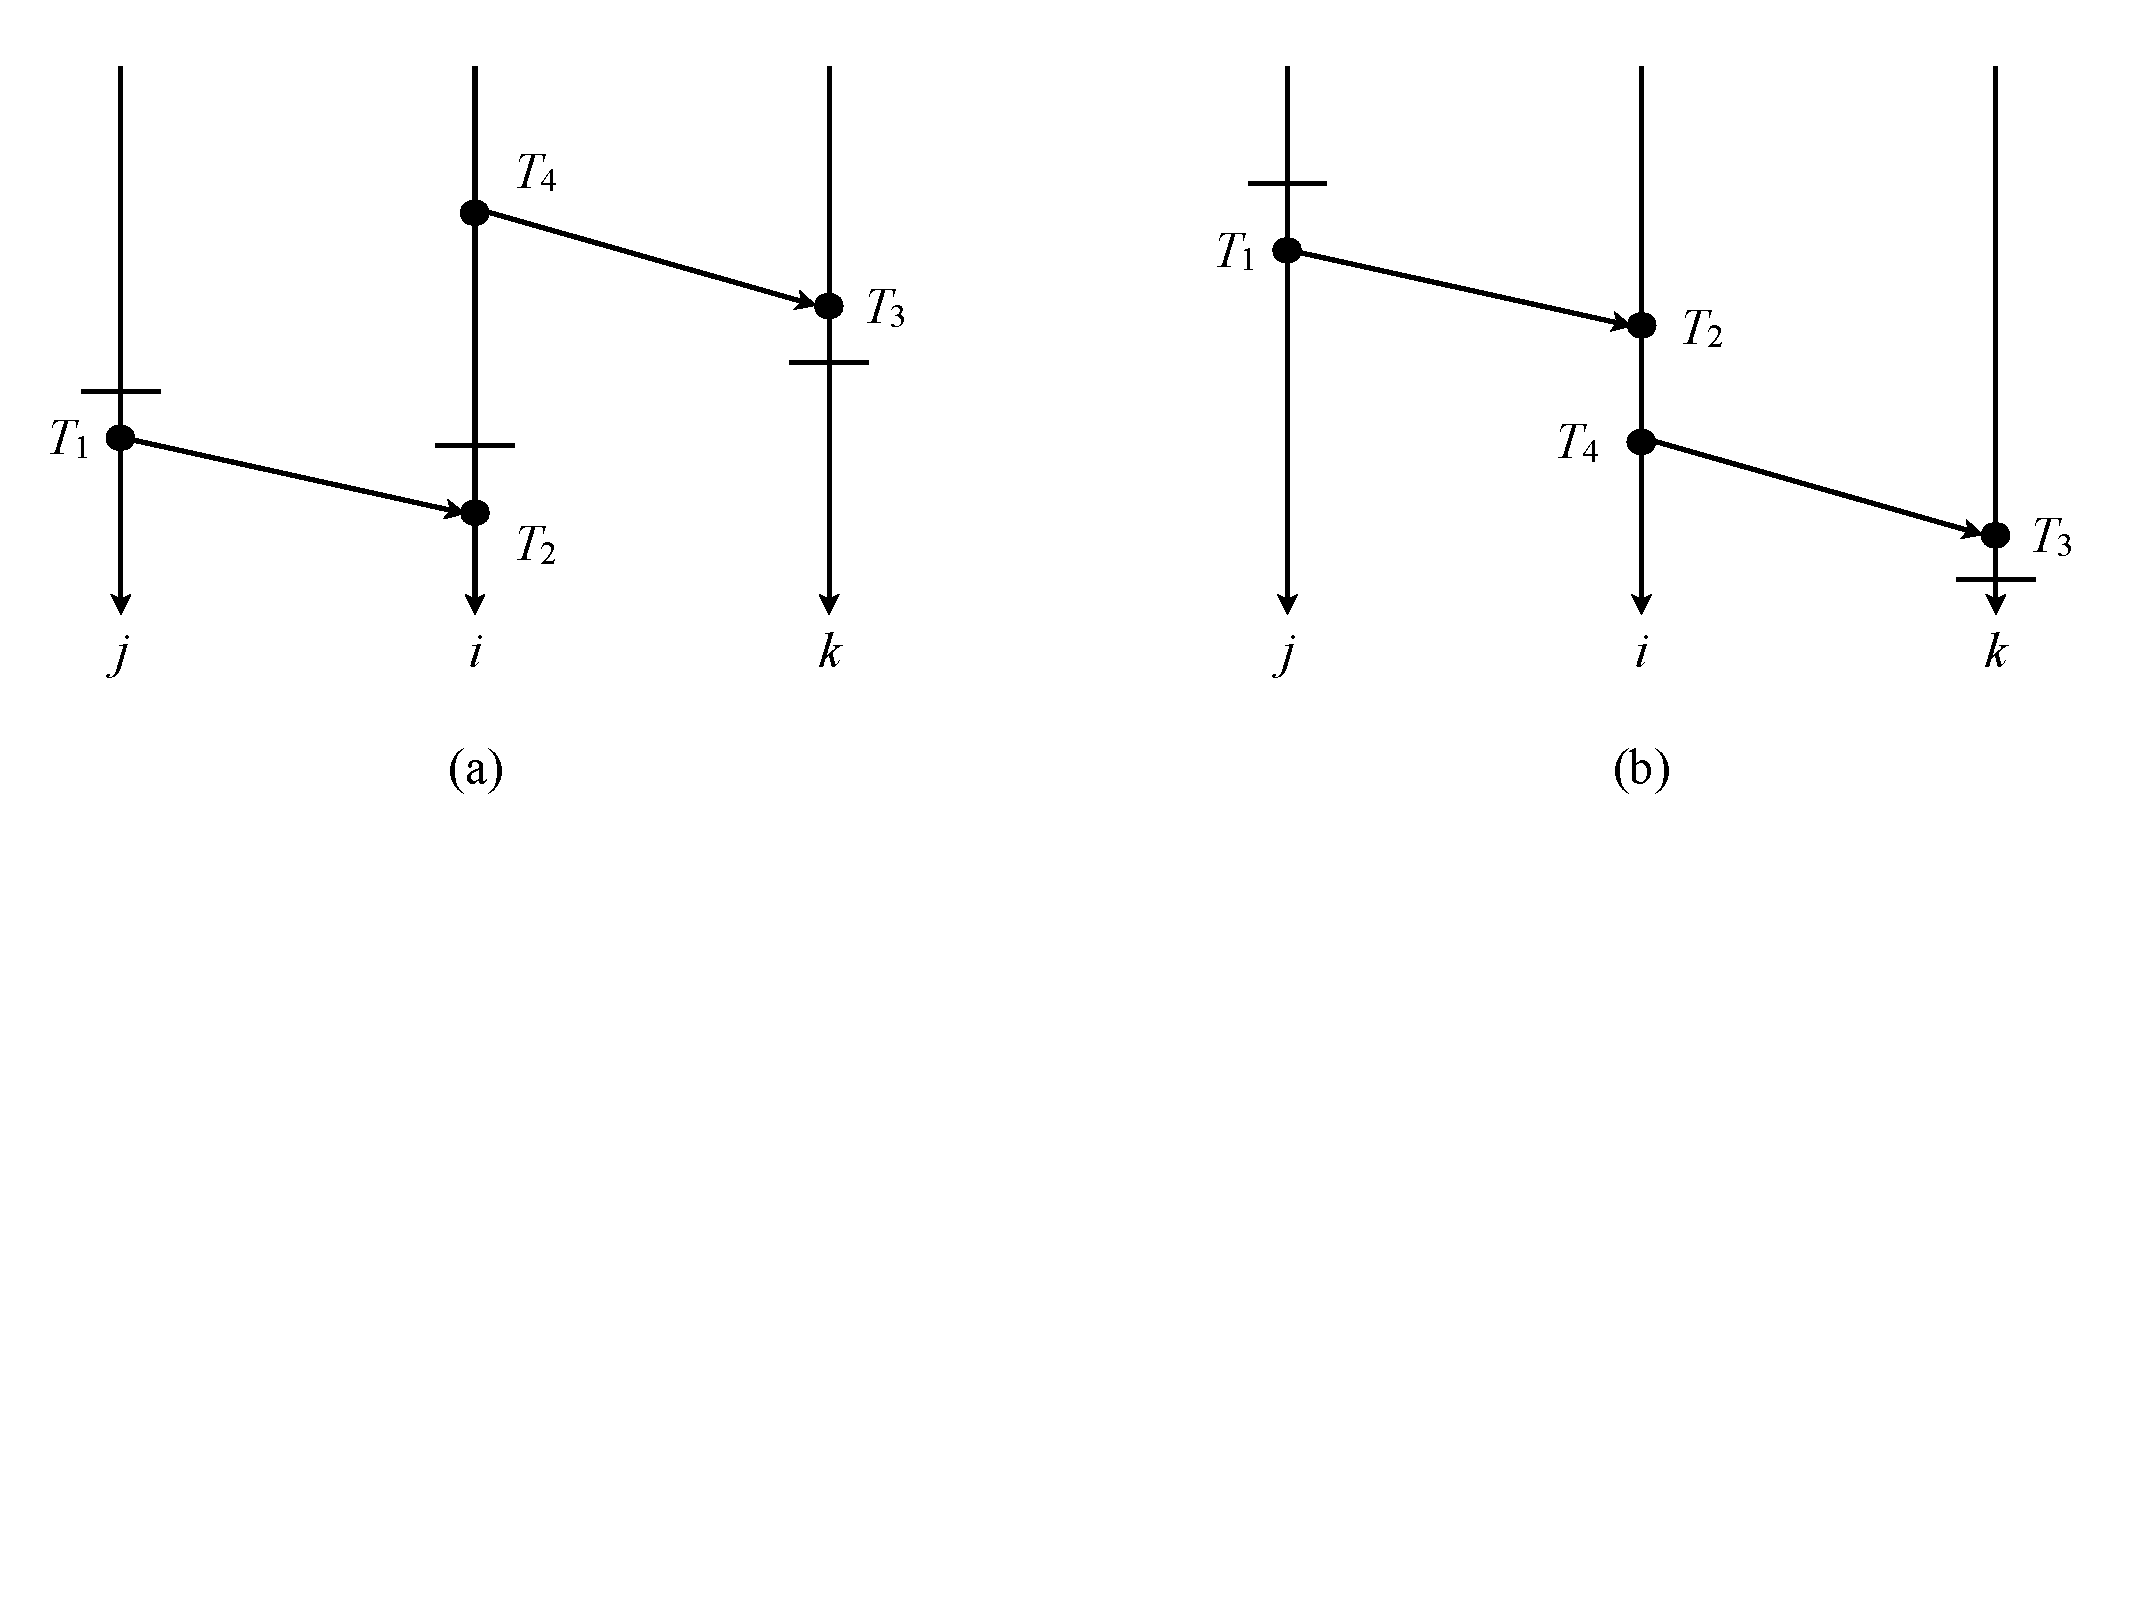
\includegraphics[width=\textwidth]{figures/ch4_snapshot.pdf}
\vspace{-6.5cm}
\caption{Illustrations of the snapshot computation. Vertical lines depict the
  commit order at the corresponding partitions (top to bottom) and horizontal
  lines the cut-offs of various snapshots. Arrows between partitions depict
  causal dependencies.}
\label{fig:snapshot}
\end{figure}

On the one hand, the snapshot cannot be too fresh. For example, suppose a transaction $\tx_1$ that wrote to partition $j$ is excluded from the snapshot chosen by $\tx$ at $j$. Then, the snapshot chosen by $\tx$ at partition $i$ cannot contain $\tx_1$, nor any other transaction that causally depends on it, like $\tx_2$ (Figure~\ref{fig:snapshot}a). If the snapshot chosen by $\tx$ included $\tx_2$, it would be able to read some of $\tx_2$'s writes at $i$, thereby forcing $\tx$ to read the writes by $\tx_2$'s causal dependencies, including $\tx_1$; but $\tx$ cannot see these writes, because it excluded them from the snapshot at partition $j$. Thus, when building the snapshot, the server needs to take into account the snapshots taken by $\tx$ at the partitions it already read; the server selects the longest prefix of $\CommitLog$ transactions, such that their writes---and the ones by their causal dependencies---are included in $\tx$'s previous snapshots. This prefix is denoted by $r$ (line~\ref{alg:max_vc_search}), and is computed using the $\Vaggr$ vector included in each of the entries of $\CommitLog$, summarising the causal dependencies of all transactions up to a given record in the log. Thus, the snapshot at $s_i$ includes all transactions with sequence numbers up to $r.\Vaggr[i]$.

On the other hand, the snapshot selected cannot be too stale. Continuing with the previous example, if a transaction $\tx_3$ is included in the snapshot taken by $\tx$ at some partition $k$, then the snapshot of $\tx$ at partition $i$ has to include the writes by $\tx_3$ and its causal dependencies, e.g., the transaction $\tx_4$ in Figure~\ref{fig:snapshot}a. The snapshot vector $\tx.\VCaggr$ summarises the updates of the transactions (and of its causal dependencies) included in the snapshots fixed by $\tx$. Thus, after determining the appropriate snapshot in line~\ref{alg:max_vc_search}, the server $s_i$ checks that this snapshot covers transactions with sequence numbers at $i$ up to $\VCaggr[i]$ (line~\ref{alg:read_req_abort_check}). To maximise the chances of passing this check, before allowing a transaction $\tx$ to proceed with a read, the server $s_i$ waits until the writes from the prefix up to $\VCaggr[i]$ have been incorporated into its state (line~\ref{alg:read_req_wait}).

It may be the case that it's impossible to satisfy both of the above requirements when selecting a snapshot; e.g., in the situation illustrated in figure~\ref{fig:snapshot}b. Assuming that the transaction $\tx$ has fixed a valid snapshot at $j$ and $k$, it is impossible to build a consistent snapshot at partition $i$; given that $\tx$ included $\tx_3$ at partition $k$, it is forced to read $\tx_4$'s writes at $i$. At the same time, because it excluded $\tx_1$ from the snapshot at $j$, $\tx$ can't read the writes by $\tx_2$ at $i$. In this case, without the second requirement, the server $s_i$ would build a snapshot excluding both $\tx_2$ and $\tx_4$, violating $T$'s causal dependency on $\tx_3$. In this case the server sends to the client a $\READRETURN$ message with a special value $\abort$ (line~\ref{alg:read_req_abort}), which will cause the client to abort the transaction (line~\ref{alg:read_abort}).

Once the server fixes a new snapshot, it selects the most recent version of the object $x$, defined by $e.\Vaggr[i]$ (line~\ref{alg:chose-version}), to return to the client. The server replies with a $\READRETURN$ message, carrying a triple of the value of the object, its associated version vector, and the aggregate vector for $e.\Vaggr$, summarising the causal dependencies of all the transactions in the snapshot. When the client receives the message (line~\ref{alg:read_msg_decomp}), it first sets the $j$-th entry of $\tx.\hasRead$ to $\top$, to indicate that $\tx$ has read an object at partition $j$, and joins the returned aggregate vector to $\tx.\VCaggr$. The client also joins the commit vector associated with the version read to a \emph{dependency vector} $\tx.\VCdep$, which represents all causal dependencies developed by $\tx$ during its execution. This ensures that, upon reading a version of object $x$, $\tx$ will causally depend on the transaction $\tx'$ that wrote that version of $x$, along with the causal dependencies of $\tx'$.

\begin{figure}[t]
\vspace{-2cm}
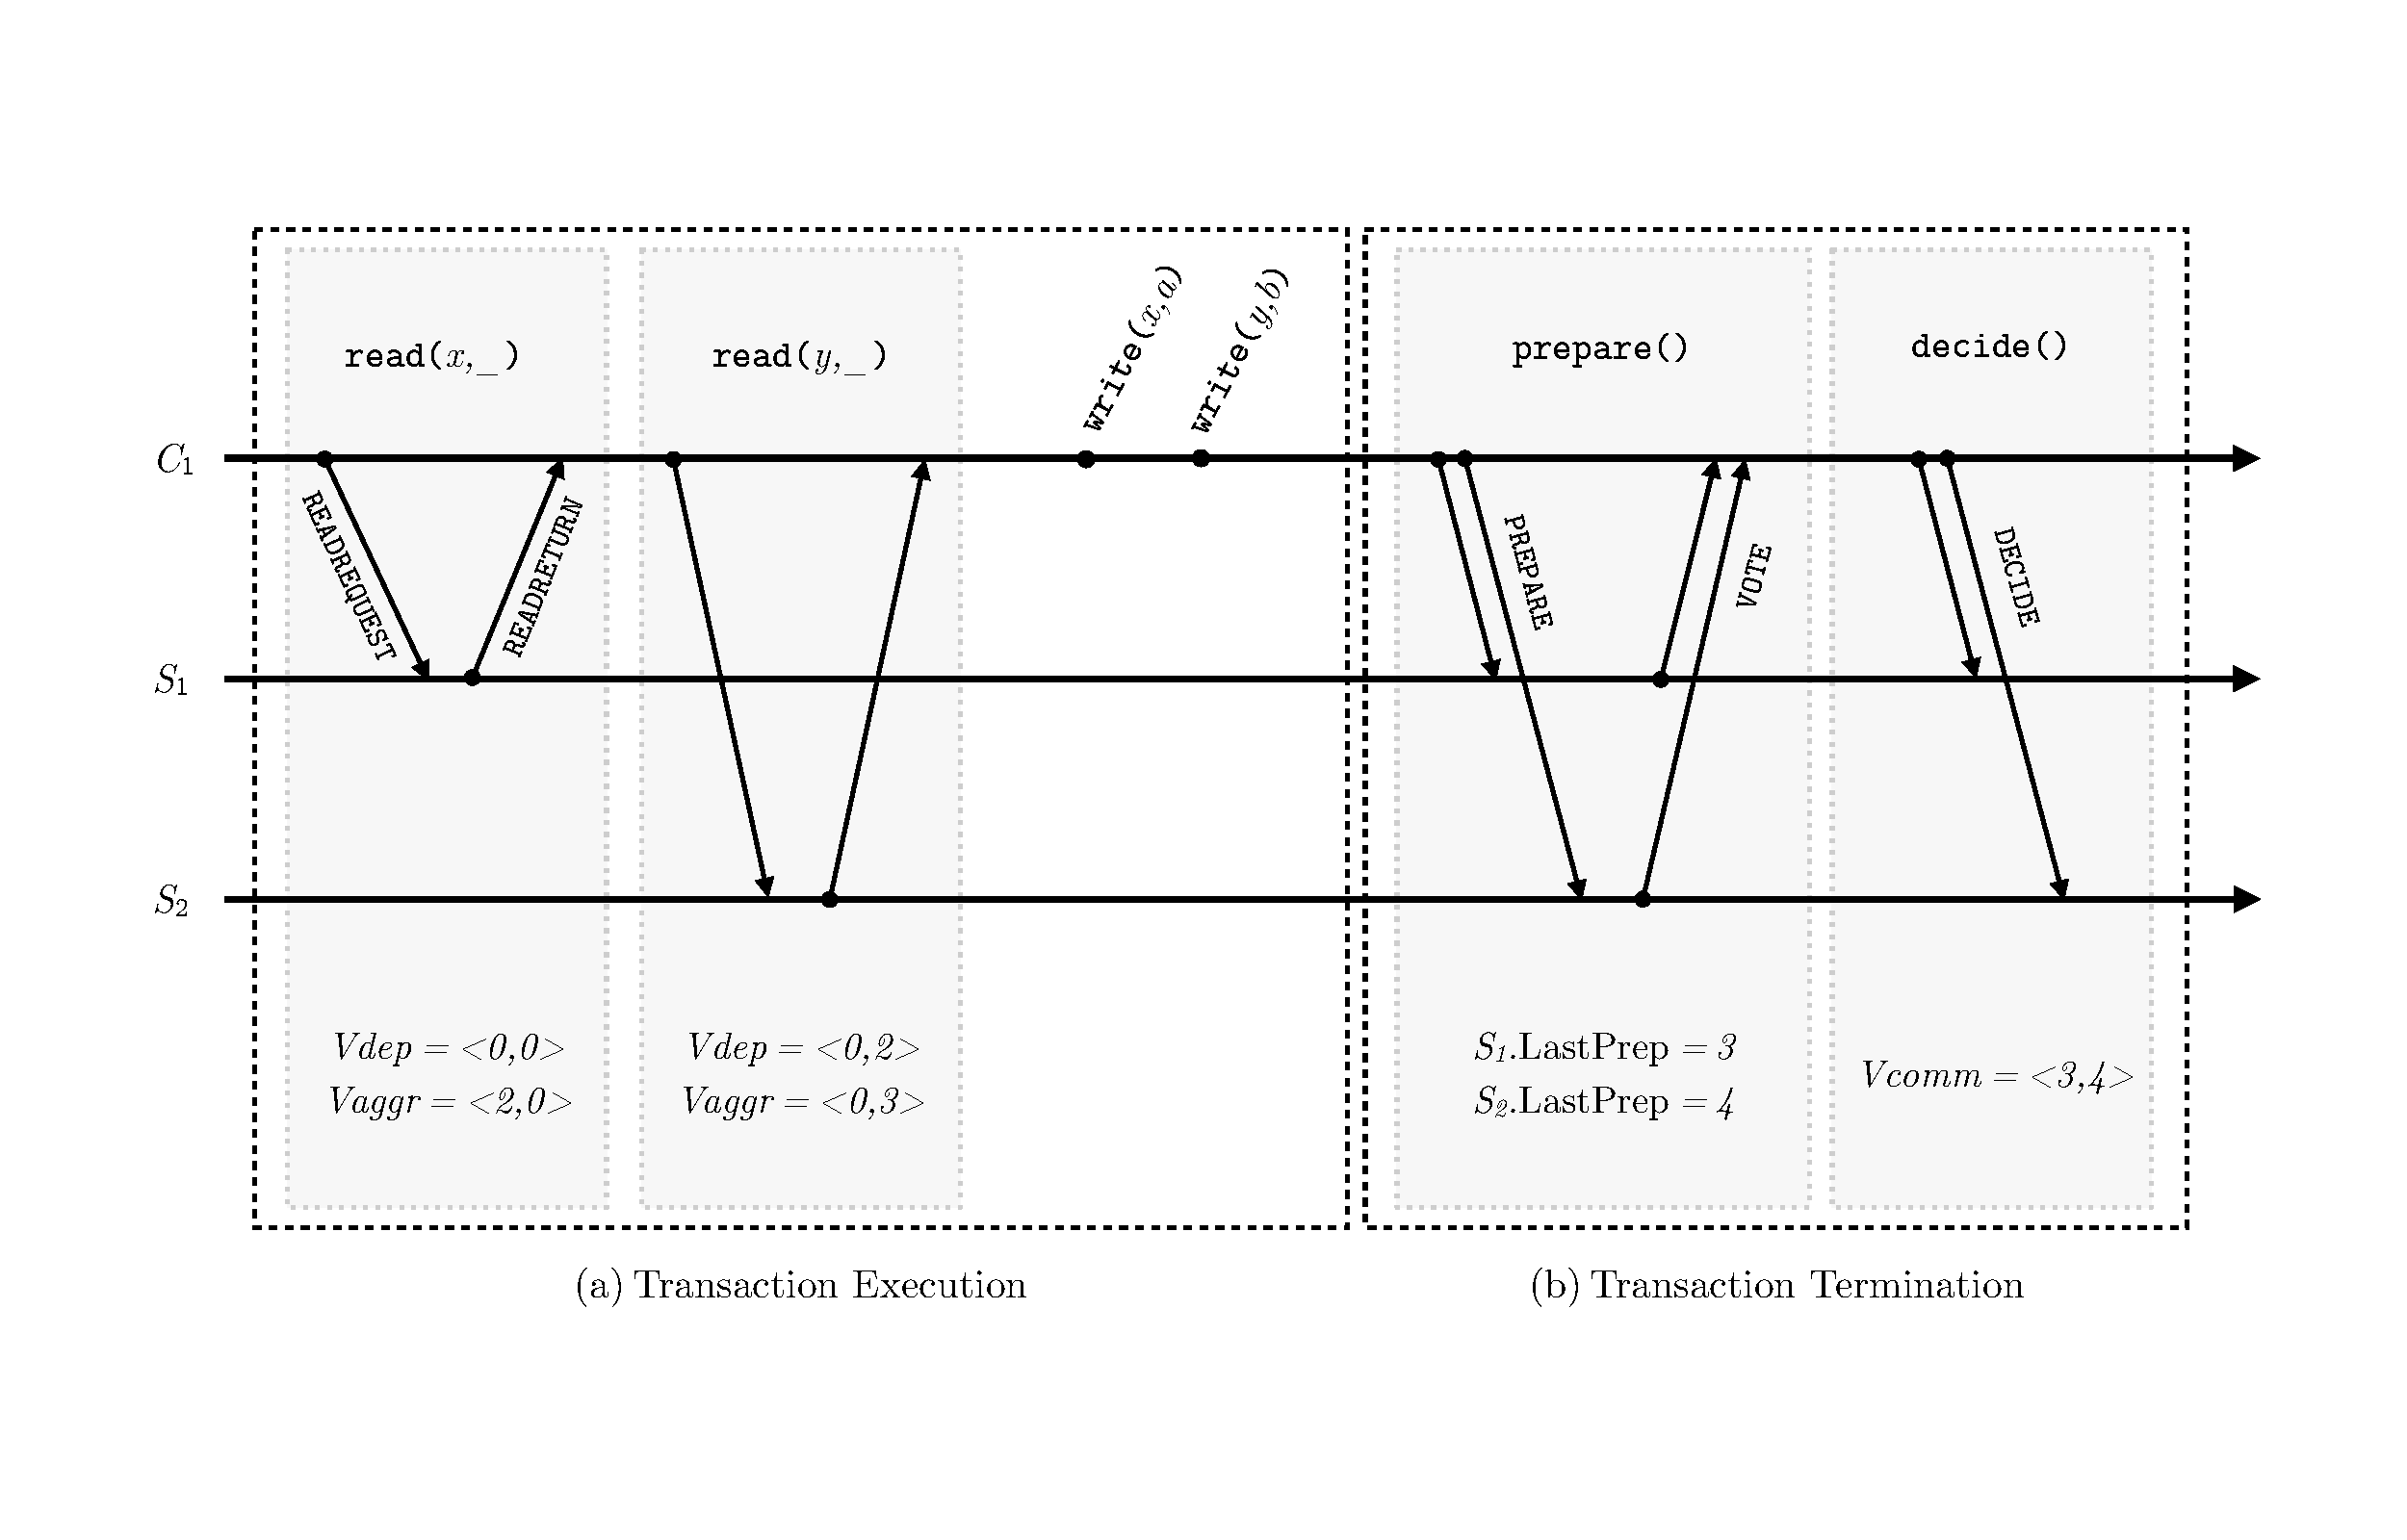
\includegraphics[width=\textwidth]{figures/ch4_execution.pdf}
\vspace{-2cm}
\caption{Message flow diagram of a sample execution, with message arrows labeled with their names in the protocol. The different interactions between a client and servers are shown in the shadowed regions. The operation performed by the client is shown at the top, and the state observed by the client at the end of each message exchange is summarised at the bottom.}
\label{fig:sample_execution}
\end{figure}

Consider the example depicted in Figure~\ref{fig:sample_execution}a, which shows a complete execution of the protocol. Client $c_1$ issues a pair of read requests to servers $s_1$ and $s_2$. In turn, these servers reply with the value of the object requested, along with its version vector and the new aggregate vector for the transaction, denoted by $\VCdep$ and $\Vaggr$ at the bottom. Since this is the first read request issued on behalf of this transaction, the server $s_1$ replies with its most recent aggregate vector, stored in $\LocalTime$. In addition, it replies with the most recently updated version of $x$---the object being read---which in this case is the empty version vector, $\vec{0}$, signalling the client that the object $x$ has never been updated before. The aggregate vector $\langle 2, 0 \rangle$ signals the client that the transaction snapshot must cover committed transactions with a sequence number at $s_1$ no larger than two, and that those transactions have no causal dependencies at $s_2$, indicated by having the entry for $s_2$ set to zero. The client incorporates these two vectors to the transaction context, and issues a new read request to $s_2$. The server, in turn, must use the transaction's snapshot vector, $\tx.\VCaggr$, to compute the snapshot of $\tx$. Following the requirements already introduced, the snapshot at $s_2$ must cover the transactions already included in $\tx$'s snapshot at $s_1$. That is, it must include transactions committed at $s_2$ with a sequence number at $s_1$ no larger than two. Since at $s_2$ no committed transactions have causal dependencies on transactions that committed at $s_1$, $s_2$ is free to return its most recent aggregate vector, equal to $\langle 0, 3 \rangle$, along with the most recent version of the object requested. The client updates the context of the transaction with the dependency and aggregate vectors sent by $s_2$, which leaves the transaction with a dependency vector equal to $\langle 0, 2 \rangle$ and a snapshot vector equal to $\langle 2, 3 \rangle$.

\subsection{Transaction Termination}

To terminate a transaction, clients submit the transaction \emph{context} to the servers for validation against both previous and concurrently executing transactions. We describe how this validation occurs by referring to the algorithms in Figures~\ref{fig:client-commit} and~\ref{fig:server-commit}.

A client executing a transaction $\tx$ tries to commit it by calling a {\tt commit} function (line~\ref{alg:commit_start}). Read-only transactions are committed without any additional checks, since they already read a causally consistent snapshot (line~\ref{alg:commit_readonly_start}). To commit an update transaction $\tx$, the client executing $\tx$ serves as the coordinator for a two-phase commit among the processes that store the objects written by $\tx$.

In more detail, to commit a transaction $\tx$, the client first sends a $\PREPARE$ message to all servers storing the objects written by the transaction (line~\ref{alg:commit_send_loop}). The message contains $\tx$'s write-set and its dependency vector $\tx.\VCdep$. When a server $s_i$ receives this message (line~\ref{alg:prepare_start}), it \emph{validates} the transaction, deciding whether it should commit or abort due to conflicting concurrent transactions. The server then replies to the client with a \emph{vote} representing its decision. Based on the votes, the client determines the final decision on the transaction---the transaction commits if all votes are positive---and distributes the decision to the relevant servers.

\begin{figure}[h]
\begin{algorithm}[H]
  % Commit
  \SubAlgo{\Fun ${\tt commit}(T)$\label{alg:commit_start}}{
    \If{$\tx.\WS = \emptyset$\label{alg:commit_readonly_start}}{
      \Return{$\commit$}\;\label{alg:commit_readonly_end}
    }

    \ForAll{$\partj \in \partitions(\tx.\WS)$\label{alg:commit_send_loop}}{
      \Send{$\PREPARE(T, T.\WS, \VCdep)$} \KwTo $\partj$\;\label{alg:commit_send_prepare}
    }

    $\commitVC \leftarrow \tx.\VCdep$\; \label{alg:commit_commitvc_firstassignment}
    $\outcome \leftarrow \commit$\;

    \ForAll{$\partj \in \partitions(\tx.\WS)$\label{alg:commit_send_votes}}{
      \Receive{$\VOTE(m)$} \KwFrom $\partj$\;\label{alg:commit_recv_vote}
      \uIf{$m = \langle T, \abort \rangle$\label{alg:commit_vote_check}}{
        $\outcome \leftarrow \abort$\;
        \Break\;
      }
      \ElseIf{$m = \langle T, \commit, k \rangle$\label{alg:commit_vote_check_else}}{
        $\commitVC[j] \leftarrow k$\;\label{alg:commit_assign_seqn}
      }
    }

    \ForAll{$\partj \in \partitions(\tx.\WS)$}{
      \Send{$\DECIDE(\tx, \commitVC,\outcome)$} \KwTo $\partj$\;\label{alg:commit_send_decide}
    }

    \Return{$\outcome$}\;\label{alg:commit_end}
  }

\end{algorithm}
\caption{Commit protocol of a transaction at client $c_i$. The client acts as a coordinator for the commit.}
\label{fig:client-commit}
\end{figure}

\begin{figure}[h]
\begin{algorithm}[H]

  % Prepare
  \SubAlgo{\WhenReceived $\PREPARE(T, \localWS, \localVdep)$ \KwFrom
    $c_j$\label{alg:prepare_start}}{
    \If{$(\exists T'.\ (\langle T', \pending, \localWS' \rangle \in \cqueue$
      \begin{tabularx}{\linewidth}{l}
        \quad\quad\quad$\vee\ \langle T', \ready, \_, \_ \rangle \in \cqueue)$\\
        \quad\quad\quad$\wedge\
        (\localWS' \cap \localWS \ne \emptyset)$\\
        $\vee \left(
          \exists x. \ x \in \localWS
          \wedge (\VersionLog[x].\last.\Vcomm[i] > \localVdep[i])\right)$\\
      \end{tabularx}\label{alg:conflict_check}
    }{
      \Send{$\VOTE(t, \abort)$} \KwTo $c_j$\; \label{alg:send_abort}
      \Return\;
    }
    $\lastprep \leftarrow \lastprep + 1$\;\label{alg:lastprep_incr}
    $\cqput(\tx, \pending, \localWS)$\;\label{alg:queue_put}
    \Send{$\VOTE(\tx, \commit, \lastprep)$} \KwTo $c_j$\;\label{alg:prepare_end}
  }

  \smallskip

  % Decide
  \SubAlgo{\WhenReceived $\DECIDE(T, \commitVC, \outcome)$ \KwFrom
    $c_j$\label{alg:decide_start}}{
    \uIf{$\outcome = \commit$\label{alg:decide_if}}{
      $\cqupdate(\langle \tx, \ready, \_, \commitVC\rangle)$\;\label{arg:queue_update}
    }
    \Else{
      $\cqremove(\tx)$\;\label{alg:decide_end}
    }
  }

  \smallskip

  % Queue head
  \SubAlgo{\Upon $\langle T, \ready, \localWS, \commitVC\rangle =
    \cqhead()$\label{alg:queue_start}}{
    \ForAll{$\{\langle x , v \rangle \mid \langle x , v \rangle \in \localWS \wedge \partitionof(x) = i\}$} { \label{alg:queue_loopws}
        $\vlapply(\langle x , v , \commitVC \rangle)$\;\label{alg:queue_vapply}
    }

    $\mrvc \leftarrow \max(\mrvc,\commitVC)$\;\label{alg:queue_mrvc}
    $\cladd(T, \mrvc)$\;\label{alg:queue_clog_add}
    $\cqremove(T)$\;\label{alg:queue_end}
  }
\end{algorithm}
\caption{Commit protocol of a transaction at server $s_i$.}
\label{fig:server-commit}
\end{figure}

We now describe how a server $s_i$ computes its vote on a transaction (line~\ref{alg:conflict_check}). The vote for a transaction $\tx$ ensures the write-conflict freedom property of PSI:

\begin{itemize}
    \item \emph{For any pair of distinct transactions $\tx_1$ and $\tx_2$ writing to an object $x$, if $\tx_1$ precedes $\tx_2$ in the commit order, then $\tx_2$ must see a version of $x$ at least as up-to-date as the one written by $\tx_1$.}
\end{itemize}

To ensure this property, the server $s_i$ first check whether, for the objects that $\tx$ updated, the versions that $\tx$ read are still the most up-to-date ones in the database of $s_i$ at the time of validation. The server then checks whether $\tx$ conflicts with any transactions present in $\CommitQueue$, which have started committing at the server, but whose writes have not been applied to the database yet (line~\ref{alg:conflict_check}). If any such transaction $\tx'$ in $\CommitQueue$ writes to the same object as $\tx$, the server should abort $\tx$. The writes of transactions in $\CommitQueue$ may be applied to the database before the writes of $\tx$, so checking for such conflicts ensures that the reads by $\tx$ will still be up-to-date when its writes are applied to the database.

If the validation for transaction $\tx$ fails, the server sends a $\VOTE$ message with the vote \abort, which tells the client to abort the transaction (line~\ref{alg:send_abort}). If the validation succeeds, the server generates a sequence number for the transaction by incrementing $\lastprep$. Then, it sends to the client a $\VOTE$ message with this sequence number and a vote \commit (line~\ref{alg:prepare_end}). The server also adds an entry $\langle \tx, \pending, \tx.\WS \rangle$ to the $\CommitQueue$, to record the fact that it is trying to commit $\tx$ at the server (lines~\ref{alg:lastprep_incr}--\ref{alg:prepare_end}).

The client waits until it receives $\VOTE$ messages from all involved servers (line~\ref{alg:commit_recv_vote}). If all the servers voted \commit, the client constructs the final commit vector for $\tx$ by changing its dependency vector $\tx.\VCdep$, so that it not only covers the updates of $\tx$'s causal dependencies, but also the updates of $\tx$. These writes are identified by the sequence numbers provided by the servers as part of their $\VOTE$ messages. Thus, the commit vector is defined by setting the entries in $\tx.\VCdep$ for partitions written by $\tx$ to these sequence numbers (line~\ref{alg:commit_assign_seqn}). The client then sends a $\DECIDE$ message to all the involved servers with the final decision on $\tx$ along with its commit vector (line~\ref{alg:commit_send_decide}).

Upon receiving a $\commit$ decision on a transaction $\tx$ (line~\ref{alg:decide_start}), a server updates the entry associated with $\tx$ in $\CommitQueue$, to change its status to $\ready$ and record its commit vector. If the transaction is aborted, the server removes $\tx$ from the queue.

Committed transactions are applied to the database in their order in $\CommitQueue$, i.e., the commit order. When a $\ready$ transaction $\tx$ gets to the head of the queue (line~\ref{alg:queue_start}), the server dequeues it and adds its writes to $\VersionLog$, tagged with its commit vector. The server then joins $\tx$'s commit vector to $\LocalTime$, and adds the transaction to $\CommitLog$, along with $\LocalTime$ as its aggregate vector.

\section{Consistency Tradeoffs and Read Aborts}
\label{sect:read_aborts}

As mentioned in \ref{subsect:protocol_execution}, a transaction $\tx$ reads a causally consistent snapshot from a partition when two properties are maintained: on the one hand, if the snapshot of $\tx$ excludes a particular transaction $\tx'$, then $\tx$ must exclude $\tx'$, together with any other transaction that causally depends on it, from the snapshots $\tx$ fixes at any other partition. On the other hand, if the snapshot of $\tx$ includes a transaction, that transaction---along with its causal dependencies---must be included in any other snapshot fixed by $\tx$ at any other partition. These two properties provide fastPSI with part of its consistency guarantees: transactions accessing objects in a single partition are executed under Snapshot Isolation (SI), whereas transactions accessing objects in different partitions are executed under Parallel Snapshot Isolation (PSI).

However, it might be that both consistency models cannot be guaranteed at the same time. Since Snapshot Isolation requires a strict order between snapshots, this means that fastPSI must provide a strict per-partition order of snapshots, which is represented by the commit order at a particular partition. At the same time, under Parallel Snapshot Isolation, partitions are allowed to commit transactions in different order, as long as those transactions are non-conflicting. When a transaction cannot build a snapshot that satisfies both consistency models, it is forced to abort.

Recall from~\ref{sect:protocol_structures} the usage of version vectors to represent causal dependencies, such that a transaction $\tx_k$ causally depends on $\tx_j$ if $\tx_j.\Vcomm \sqsubseteq \tx_k.\VCdep$, i.e., $\tx_k$ is causally dependent on $\tx_j$ if $\tx_k$ observes the updates of $\tx_j$. At the same time, the commit order of transactions at a partition $i$ is derived from the sequence numbers of transactions at $i$, such that $\tx_j$ committed before $\tx_k$ if $\tx_j.\Vcomm[i] < \tx_k.\Vcomm[i]$.

In practice, since the dependency vector $\VCdep$ of a transaction is used as the initial value of its commit vector (line~\ref{alg:commit_commitvc_firstassignment}), this makes any two transactions committing at the same partition causally dependent on each other, even if they are not aware of each other's updates. Nevertheless, this causal dependency is only established after both transactions are committed, and thus it doesn't interfere in their validation process.

% However, when a transaction $\tx$ fixes a snapshot at partition, the possible causal dependencies of $\tx$ are computed according to its snapshot vector, $\tx.\VCaggr$, which represents the join of the commit vectors of transactions that committed at the partitions that $\tx$ read before. In practice, this means that for the purposes of fixing a snapshot, two transactions $\tx_1$ and $\tx_2$ are considered to be causally dependent if $\tx_1.\Vcomm \sqsubseteq \tx_2.\VCaggr$, i.e. $\tx_2$ causally depends on $\tx_1$ if it is included in $\tx_2$'s snapshot.

This limitation comes from the strict per-partition commit order requirement of SI and from the coarse-grained nature of version vectors. When combined with the property of PSI that allows different commit orders across partitions, it can cause situations such that any snapshot that observes a particular order of transactions will not be causally consistent. When this happens, any transaction that observes such order will need to abort.

\begin{figure}[t]
\centering
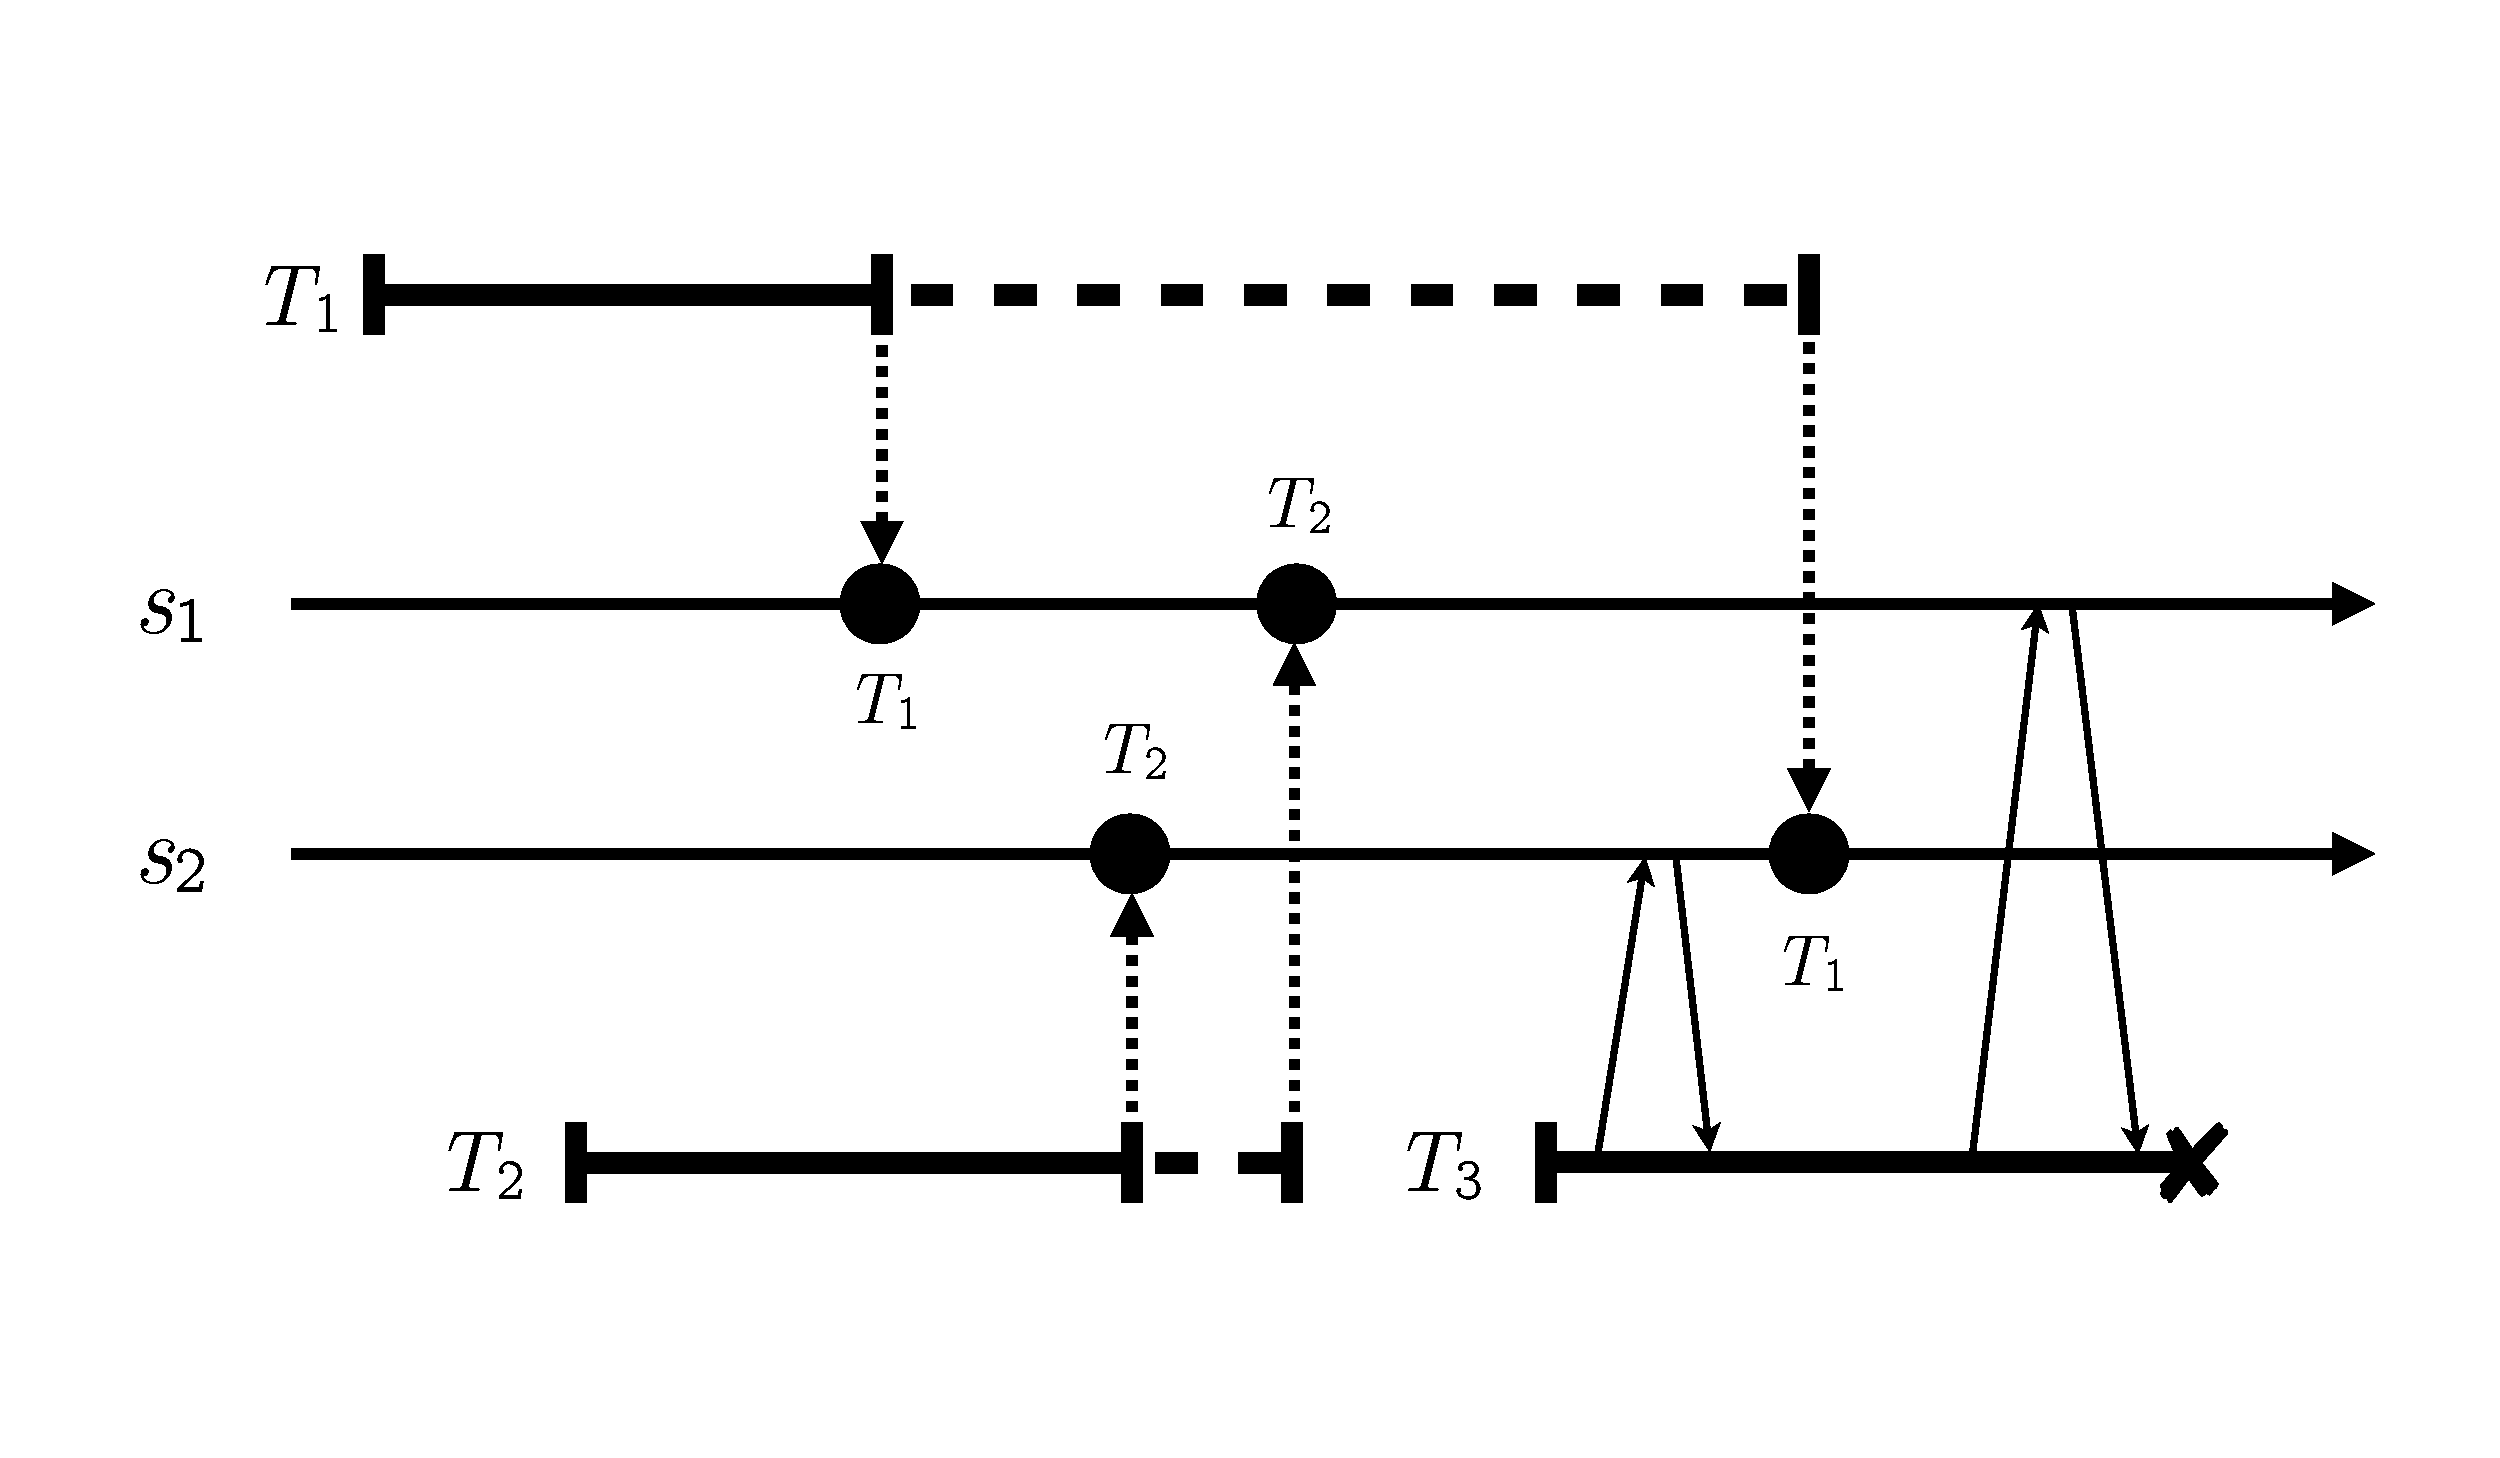
\includegraphics[width=0.6\textwidth]{figures/ch4_abort_execution.pdf}
\vspace{-0.5cm}
\caption{Example read abort execution. Bold horizontal lines represent executions of transactions over time (left to right), the black circles represent the commit times of the transactions at different servers, and the dotted bold lines represent time it takes for the commit of a transaction to propagate to the other servers. Arrows between transactions and servers represent messages. The cross in the execution of $\tx_3$ marks its abort time. }
\label{fig:read_abort}
\end{figure}

The example in Figure~\ref{fig:read_abort} illustrates such an order, with $\tx_1$ and $\tx_2$ being a pair of concurrent, non-conflicting transactions, both committing at servers $s_1$ and $s_2$. Due to the strict per-partition order requirement inherited from SI, both servers order $\tx_1$ and $\tx_2$ according to their local sequence number. In addition, the weaker consistency guarantees of PSI allow servers to commit transactions in different order, such that $s_1$ observes $\tx_1 \hb \tx_2$, and $s_2$ observes $\tx_2 \hb \tx_1$. Usually, this divergence in the commit order of transactions doesn't affect the ability of subsequent transactions to form a causally consistent snapshot: as long as a transaction is able to observe both $\tx_1$ and $\tx_2$ at every partition, their respective commit orders are irrelevant. However, consider the execution of $\tx_3$ in Figure~\ref{fig:read_abort}. The transaction reads an object from server $s_2$, including $\tx_2$ in its snapshot; however, the read operation of $\tx_3$ arrives at $s_2$ before the commit of $\tx_1$ propagates to the server, and therefore $\tx_3$ excludes $\tx_1$ from its snapshot. Following this, $\tx_3$ attempts to read an object from $s_1$. Since $\tx_3$ included $\tx_2$ in its snapshot at $s_2$, it must also include it in its snapshot at $s_1$; on the other hand, since $\tx_3$ excluded $\tx_1$ at $s_2$, its snapshot must not include $\tx_1$ at $s_1$. However, due to the fact that $s_1$ observed the order of both transactions as $\tx_1 \hb \tx_2$, the two requirements to form a causally consistent snapshot for $\tx_3$ are contradictory: including $\tx_2$ in its snapshot would force $\tx_3$ to observe $\tx_1$, whereas excluding $\tx_1$ would force $\tx_3$ to also exclude any other transaction that causally depends on $\tx_1$, i.e., $\tx_2$. In this situation, $\tx_3$ cannot form a causally consistent snapshot at $s_1$, and thus it must abort.

   \cleardoublepage
\chapter{Implementation and Evaluation}
\label{chapter:evaluation}

We now offer an evaluation that attempts to explore the overhead of the stronger consistency model of fastPSI, compared to the weakest consistency model that satisfies the atomicity of transactions, namely Read Committed. We also show how fastPSI is able to outperform a protocol implementing the stronger Serialisability consistency model. Finally, we evaluate the scalability of fastPSI as more servers and partitions are added to the system, and discuss some of the weak points of the protocol.\todonote{rephrase?}

\section{Implementation}

Our implementation of the fastPSI protocol consists of a client-side library~\citep{pvc-client} and a server~\citep{pvc-server}, the latter being written as a plug-in transactional protocol for Antidote~\citep{antidote-db}, a reference platform for evaluating consistency protocols. Both the client library and the server are written in the Erlang programming language, with a total of 6K lines of code. The Antidote platform provides a key-value database, supports both in-memory and disk-based storage, and implements full replication. For simplicity, our implementation only supports in-memory storage, and lacks a replication mechanism. The client-side library communicates with the server using Google's Protocol Buffers~\citep{protobuf}. To enhance network efficiency, client messages are transmitted in periodic batches to the servers.

To validate the results of our evaluation, we also implement two alternative protocols satisfying the Read Committed and Serialisability consistency models, called \textbf{naiveRC} and \textbf{naiveSER}, respectively. Both are built on top of our original implementation and are as efficient as possible. The pseudocode for both implementations can be found in Appendix~\ref{appendix:code}.

Given that fastPSI requires the use of multiple versions per object, it becomes necessary to prevent an unbounded growth of the number of versions in the $\VersionLog$ database, and in the number of entries in the per-partition $\CommitLog$. We implement a simple garbage collection mechanism that maintains a fixed number of versions and that regularly prunes the oldest versions from the state of a partition.\todonote{Mention tradeoff w/ number of versions and abort ratio?}

\section{Evaluation}

We evaluate the performance of fastPSI using the Yahoo! Cloud Serving Benchmark~\citep{ycsb}, modified to generate transactional workloads~\citep{ardekani_nmsi, ardekani_gdur}. Our implementation of Read Committed is used as a baseline for comparison, in order to show the maximum possible performance. Figure~\ref{fig:workload-types} describes the workloads used\todonote{mention that D and E are invented. Maybe say that we take inspiration from YCSB, instead of saying that we use it}. All experiments are run on a cluster consisting of machines with 3.80~GHz to 4.70~GHz Intel Xeon processors with six cores, 32~GB of RAM, and a single 1~Gbps network port. We partition the cluster in up to three different sites, with four server machines and four client machines in each site. Thus, there is no shared memory between clients and servers, as if clients were acting as proxies in the same data centre as servers. Since all our machines are located in the same local network, we artificially add latency between sites using the \texttt{tc} Linux command.

In all our benchmarks, the system is loaded with one million random keys and 256-byte values prior to receiving any operations from the clients. Partitions are distributed uniformly across servers, such that a server might be responsible for multiple partitions. Keys are mapped to partitions using consistent hashing, with clients being aware of the distribution of keys to partitions and server machines. Thus, clients can directly address the correct server and partition for a specific key. Each client machine spawns multiple concurrent threads that execute transactions and communicate with servers in a closed-loop fashion. When transactions read more than object, clients perform those operations serially. For the experiments that involve more than one site, the latency between sites is of 10~ms.

\begin{figure}[h]
\begin{center}
\begin{tabularx}{0.85\linewidth}{ c | c | >{\centering}X | >{\centering}X }
    & \multirow{2}{*}{Key Selection Distribution}
    & \multicolumn{2}{c}{Operations}
\tabularnewline
    & & Read-Only Tran.
    & Update Tran.
\tabularnewline
    \hline
    % A & Zipfian & 4 Reads & 2 Reads, 2 Updates \tabularnewline
    B & Uniform & 4 Reads & 3 Reads, 1 Update \tabularnewline
    C & Uniform & 2 Reads & 1 Read, 1 Update \tabularnewline
    D & Uniform & 3 Reads & 3 Reads, 1 Update \tabularnewline
    E & Uniform & 3 Reads & 3 Reads, 3 Updates \tabularnewline
\end{tabularx}
\end{center}
\caption{Transactional YCSB Workload Types.}
\label{fig:workload-types}
\end{figure}

\subsection{Performance \& Scalability Limits}

\paragraph{Performance.} We begin by investigating the overall performance profile of our implementations. We measure and compare the throughput and latency of the different protocols as the number of update transactions increases, while keeping the number of sites constant. For this experiment, we vary the number of concurrent client threads such that we never saturate the CPU of servers. We aim to explore the overall overhead of fastPSI in comparison with naiveRC, as well as the performance benefits it offers in comparison with naiveSER. Figure~\ref{fig:general_bench} shows the results of using Workload C and three sites, with 64 partitions uniformly distributed across sites. We vary the ratio of read-only to update transactions, from 90\%/10\% to 70\%/30\% (left to right), and measure the termination latency of update transactions, i.e., the amount of time spent on the validation process of a transaction. Since the latency is measured in the client, it only reflects the amount of time spent on the \emph{prepare} phase of the commit validation, as the client does not need to wait until the changes of a transaction are committed to the partition state.

\begin{figure}[t]
\vspace{-0.5cm}
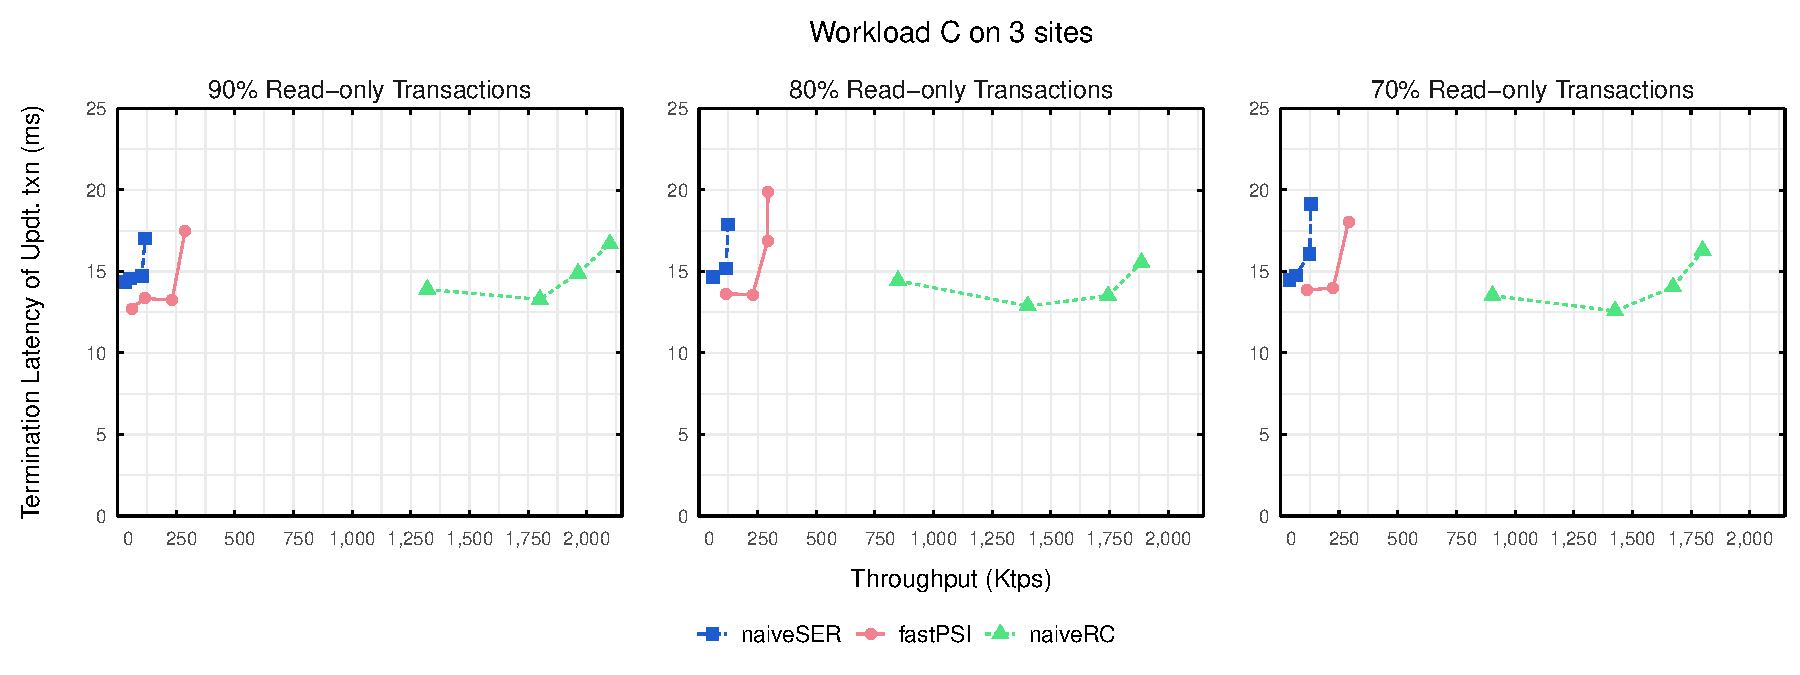
\includegraphics[width=\textwidth]{figures/general_bench.pdf}
\vspace{-1cm}
\caption{Comparison of throughput and termination latency of update transactions. \todo{Move legend to top, remove title?}}
\label{fig:general_bench}
\end{figure}

Transactions as executed by naiveRC need minimal synchronisation during its commit phase, and no synchronisation at all during read operations. This is reflected in its high performance, with the validation of update transactions as the only bottleneck in the system. Thus, as the proportion of update transactions increases, the impact on overall throughput is pronounced, dropping by as much as 20\%.

For both naiveSER and fastPSI, read operations from a transaction $\tx$ must wait until the causal dependencies of $\tx$ commit at a particular partition, bounded in the worst case by the maximum latency across sites. In addition, read operations accessing the same partition suffer from having to synchronise while fixing a snapshot, as the implementation of $\CommitLog$ is not thread-safe. These two shortcomings explain the overall low throughput in comparison with naiveRC. Nevertheless, both implementations exhibit stable performance as the proportion of update transactions increases.

By comparing fastPSI with naiveSER, we observe that the latter implementation is limited by its need to validate every transaction, in comparison with fastPSI, which only validates update transactions. In addition, the weaker consistency model offered by fastPSI allows it to outperform naiveSER in all cases by approximately 150\%, while showing similar latencies.

\paragraph{Scalability.} To explore the overall scalability of fastPSI, we examine how the maximum performance of each protocol changes as we increase the number of machines in the system. We use Workload B with a fixed ratio of 10\% update transactions, and vary the number of sites from one to three, while keeping the number of partitions fixed to 64. Figure~\ref{fig:site_bench} shows the overall performance of the protocols.

\begin{figure}[h]
\begin{center}
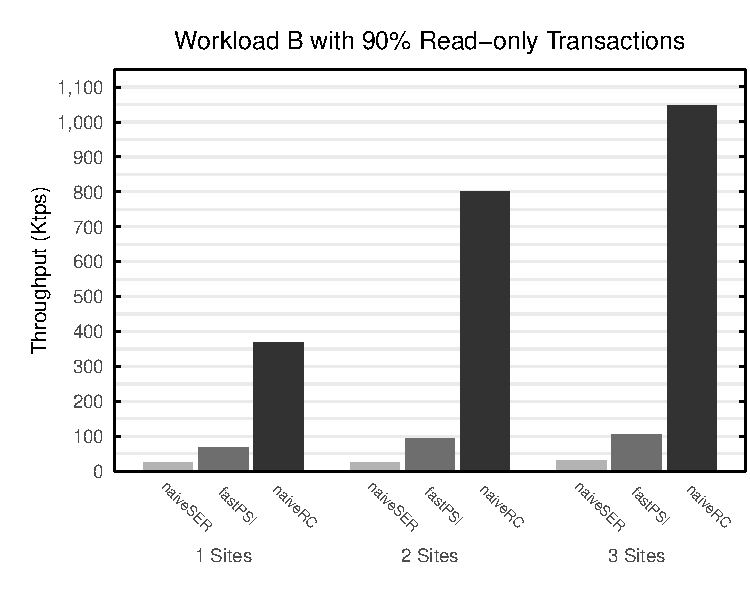
\includegraphics[width=0.5\textwidth]{figures/sites_bench.pdf}
\vspace{-1cm}
\end{center}
\caption{Maximum Throughput of Consistency Models.}
\label{fig:site_bench}
\end{figure}

As before, the performance of naiveRC increases almost in a linear fashion as we add more servers, as explained by its minimum need for synchronisation. Although the scalability of fastPSI is limited by the fixed number of partitions, it benefits moderately from increasing the number of machines: as the overall number of partitions per machine decreases, servers free resources, and can thus fulfil more client requests. This is reflected in its performance at three sites being 1.52 times its base throughput at a single site. In contrast, the overall performance of naiveSER stays almost constant as we increase the number of sites, reflecting its need to validate every transaction, which requires greater levels of synchronisation as the number of machines increases.

As the number of sites increases, so does the difference between naiveSER and fastPSI. Overall, fastPSI manages to outperform naiveSER by a factor of 2.88 with a single site, and by a factor of 3.52 at three sites.

\begin{figure}[h]
\begin{center}
\begin{tabularx}{0.75\linewidth}{ l | >{\centering}p{5cm} | >{\centering}X }
   \textbf{Parameter} &\textbf{Range} &\textbf{Default}
\tabularnewline
    \hline
    Sites & 1--3 & 3
\tabularnewline
    Update Tran. Proportion & 10\%--30\% & 10\%
\tabularnewline
\end{tabularx}
\end{center}
\vspace{-0.5cm}
\caption{Parameter space used in the comparison workload.}
\label{fig:dynamic_parameters}
\end{figure}

\begin{figure}[t]
\begin{center}
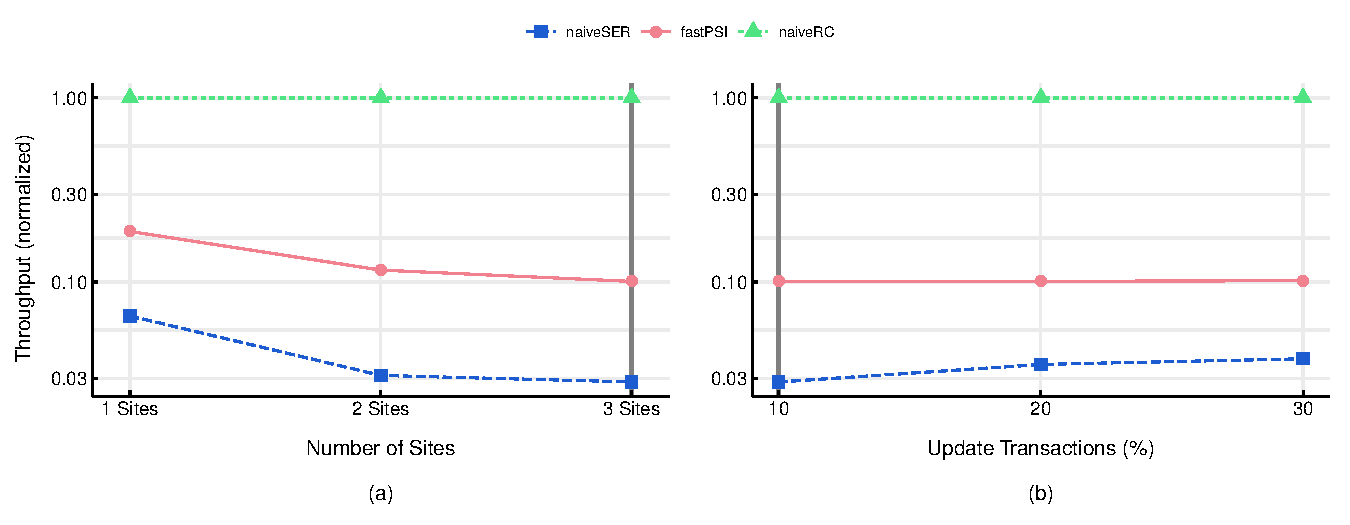
\includegraphics[width=0.8\textwidth]{figures/dynamic_bench.pdf}
\vspace{-0.75cm}
\end{center}
\caption{Parameter space exploration to reflect the performance comparison of the protocols. Each experiment varies one parameter while keeping the other fixed at its default value (represented by the grey vertical line). Throughput is shown normalised compared to naiveRC.}
\label{fig:dynamic_bench}
\end{figure}

\paragraph{Overall comparison.} We've seen how the performance and scalability of the implementations is determined by the proportion of update transactions and the number of sites. To better visualise the relationship between workload choice and performance, we explore the parameter space described in Figure~\ref{fig:dynamic_parameters} when using Workload B. As in the previous experiment, we keep the number of partitions constant as we increase the number of sites. The results are shown in Figure~\ref{fig:dynamic_bench}, with the throughput depicted normalised compared to the performance of naiveRC.

As shown in Figure~\ref{fig:dynamic_bench}a, fastPSI and naiveSER have different scalability properties. Although both implementations suffer in comparison with naiveRC, fastPSI exhibits much better scalability in comparison with naiveSER. For naiveSER, the need to validate every transaction imposes a performance penalty that increases as we add more sites, and consequently increases the overall latency of the commit phase for every transaction. In contrast, the impact on fastPSI is less severe, as the increased latency only affects the read operations, since the proportion of update transactions is low.

Figure~\ref{fig:dynamic_bench}b shows the performance comparison as the proportion of update transactions increases. While the difference in throughput between naiveRC and fastPSI stays constant, the overall performance of fastPSI is hindered by the need to compute a causally compatible snapshot. Nevertheless, the fact that the relative performance stays constant in comparison with naiveRC shows that the impact of the validation process does not grow with the number of update transactions. The impact of update transactions on naiveSER is less pronounced, and its performance difference with fastPSI gets smaller as the proportion of updates increases. This is explained by the choice of workload: read-only transactions perform four reads, while update transactions perform three. Since naiveSER also validates read-only transactions, as the proportion of update transactions grows, the average number of partitions that participate in the voting phase shrinks from four to three, which decreases the runtime cost of validation.

\subsection{Abort Ratio}

We now focus on another advantage of the relaxed consistency model of fastPSI in comparison with serialisability, namely, the ratio of aborted transactions. One of the advantages of fastPSI is that the snapshots of transactions exhibit \emph{forward freshness}: a transaction $\tx$ is able to read object versions written by transactions that committed after $\tx$ started. In contrast, a transaction $\tx$ under Serialisability or classical Snapshot Isolation can only read versions written by transactions that commit before $\tx$'s start time. This limitation leads to a high number of aborted transactions in high latency settings, due to stale reads.

\begin{figure}[t]
\begin{center}
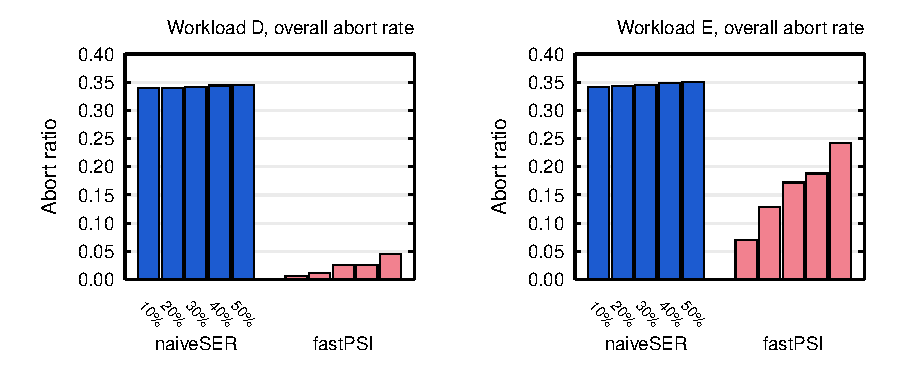
\includegraphics[width=0.8\textwidth]{figures/abort_rate_bench_overall.pdf}
\vspace{-0.75cm}
\end{center}
\caption{Overall transaction abort ratio for different consistency models and workloads.}
\label{fig:raw_abort_rate_overall}
\end{figure}

In this section, we aim to explore the advantages of forward freshness in fastPSI in comparison with naiveSER, and how different workloads affect it. In Figure~\ref{fig:raw_abort_rate_overall}, we show how the abort ratio of transactions varies---under different workloads---with the number of update transactions. The results were obtained with two sites. The graph on the left shows the advantages of the forward freshness of transactions, with the abort ratio of fastPSI being 30\% better than naiveSER, on average. However, as the number of update transactions increases, so does the number of conflicting transactions. This is reflected in an increase of aborted transactions, from less than one percent to around five percent. The graph on the right, however, shows different results: as the number of update transactions grows, so does the overall abort ratio of fastPSI, from 7\% to 25\%. Overall, in the worst case the abort ratio of fastPSI is only 10\% better than naiveSER.

To understand the difference between workloads, we turn to the two graphs depicted in Figure~\ref{fig:raw_abort_rate_2pc}, which explore the reasons why transactions abort. In fastPSI, a transaction might abort for two reasons: by updating an object that is overwritten by a concurrent transaction, or by failing to form a causally consistent snapshot, as detailed in~\ref{sect:read_aborts}. By virtue of having the same implementation of causally consistent snapshots, naiveSER inherits the same reasons, and adds a third: if a transaction reads a version of an object that is later overwritten, it is forced to abort. For both protocols, we say that a transaction might abort at two points during its execution: read aborts occur when a transaction fails to fix a causally consistent snapshot, and otherwise we say that the transaction aborts during validation, i.e., during the termination of the transaction. On the left, we see that for Workload D, all aborted transactions in fastPSI do so during the validation phase, while for naiveSER, only a small percentage of aborted transactions (between 0.5\% and 2.5\%) do so during termination. In contrast, fastPSI exhibits a very different behaviour with Workload E, as shown in the graph on the right. With this workload, transactions abort for the same reason in both protocols: they are unable to build causally consistent snapshots. In both cases, the amount of transactions that abort while attempting to fix a snapshot grows as the number of update transactions increases.

\begin{figure}[t]
\begin{center}
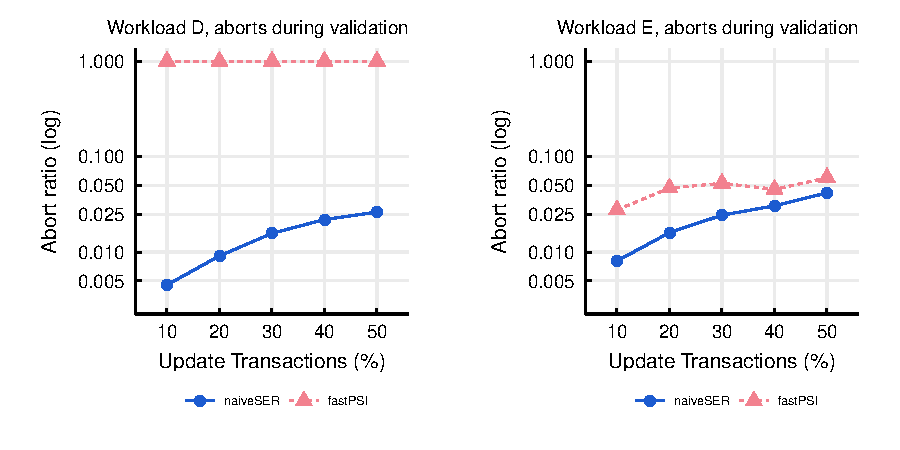
\includegraphics[width=0.8\textwidth]{figures/abort_rate_bench_2pc.pdf}
\vspace{-0.75cm}
\end{center}
\caption{Ratio of aborts that happen during the validation phase, for different consistency models and workloads.}
\label{fig:raw_abort_rate_2pc}
\end{figure}

Recall that in Workload D, update transactions update one single key, while in Workload E, they update three. This small difference in the number of update keys explains the difference in aborted transactions for fastPSI. As described in~\ref{sect:read_aborts}, a transaction $\tx$ will be unable to fix a causally consistent snapshot when a) different partitions commit non-conflicting transactions in different order, and b) $\tx$ fixes a snapshot in one of those partitions before the updates of all the non-conflicting transactions become visible. Since update transactions in Workload D only update a single key, update transactions will only commit at a single partition, and therefore, no transaction can observe a different commit order. This explains why there are no aborted transactions due to inconsistent snapshots when executing this workload for fastPSI. In contrast, update transactions in Workload E update three keys, and therefore commit at three different partitions,\footnote{Since transactions choose keys following an uniform distribution, most keys will be managed by distinct partitions.} such that the probability of partitions committing transactions in different order grows. In addition, since transactions read three keys, the probability of observing different commit orders also grows. Thus, as we increase the number of update transactions, so does the probability of transactions attempting to fix inconsistent snapshots. In naiveSER transactions also commit at the partitions they read from, meaning that update transactions in Workload D commit at three partitions. This explains why its abort ratio of  is similar in both workloads.

\begin{figure}[t]
\begin{center}
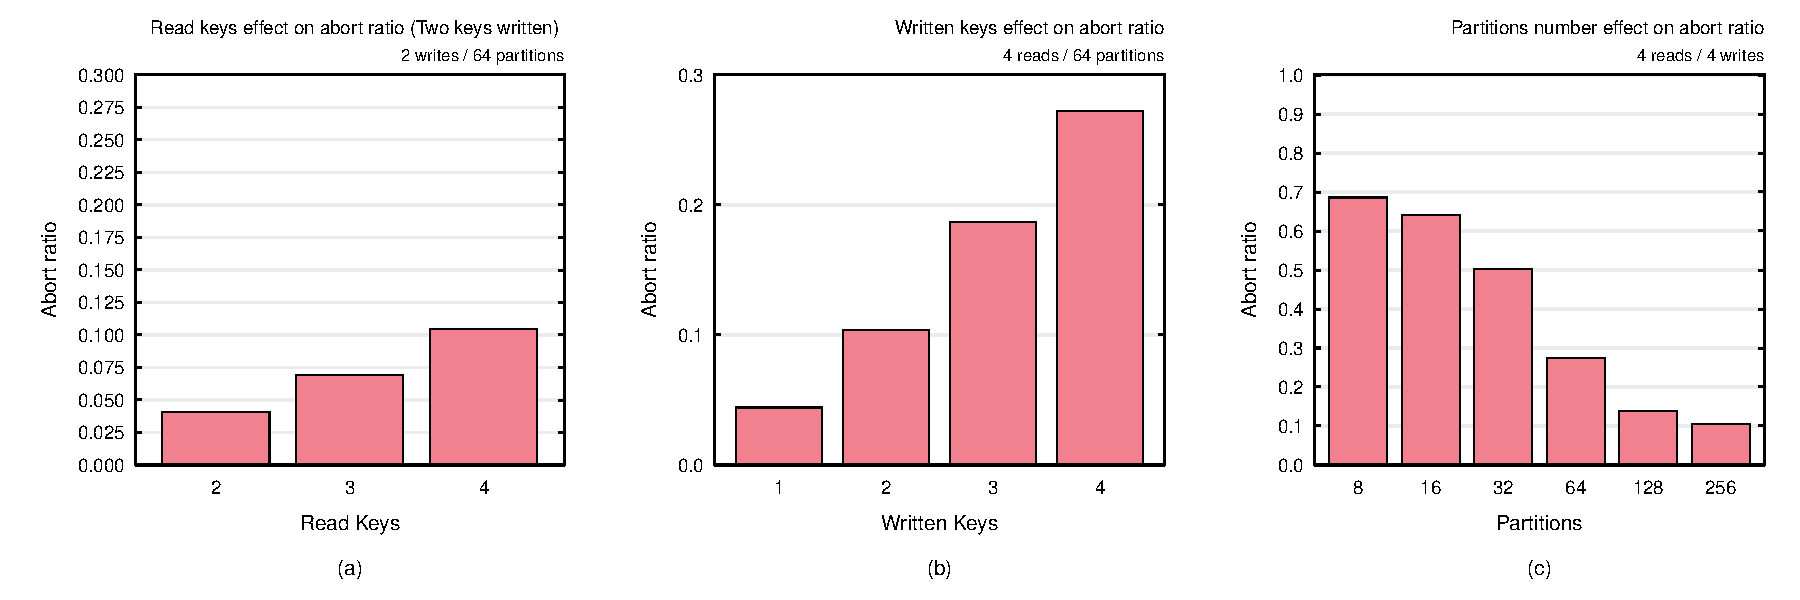
\includegraphics[width=\textwidth]{figures/psi_read_abort_bench.pdf}
\vspace{-1cm}
\end{center}
\caption{Results from exploring the abort rate of fastPSI across different workload and deployment scenarios.}
\label{fig:fastpsi_abort_rate}
\end{figure}

Since small changes in workload choice are able to affect the overall abort ratio of fastPSI in a significant manner, we finish our evaluation with an exploration of the parameters that have the highest impact on the number of aborted transactions. As explained previously, one of the reasons why transactions observe inconsistent snapshots is because partitions commit transactions in different orders. Thus, by changing the number of keys updated by a transaction, we can modify the number of partitions involved, which affects the chances of different commit orders. Another reason for inconsistent snapshots is that transactions are able to observe the transactions that commit in different order, which leads us to change the number of keys read by the transactions. If transactions read from a small amount of partitions, the probability that they observe different commit orders will also be small. Finally, the most important factor is the number of partitions, or rather, the amount of keys per partition. When a few partitions manage all the keys, most transactions will commit at the same partitions. Therefore, the probability of having different commit orders grows, as well as the probability that a given transaction observes those orders. Conversely, when the number of partitions is large, or partitions manage only a small amount of keys, the probability of different commit orders shrinks, as does the probability of them being observed by transactions.

Figure~\ref{fig:fastpsi_abort_rate} shows the results of modifying each of the parameters we mentioned, noting that we use a single site for simplicity, and modify the number of partitions, instead of changing the total amount of keys in the database. The percentage of update transactions is set to 50\%, to show the worst possible abort ratio. The effect of changing the number of keys read by a transaction, shown in Figure~\ref{fig:fastpsi_abort_rate}a, is small. Although the overall abort ratio never grows larger than 10\%, modifying the number of read keys results, at best, in an improvement of 7.5\%. Since we don't allow blind updates, the minimum number of read keys is two, since we need to update at least two keys in two different partitions to introduce inconsistent snapshots in the system. In contrast, changing the number of keys updated by a transaction produces a bigger impact, as shown in Figure~\ref{fig:fastpsi_abort_rate}b, with an overall change of 23\% in the number of aborted transactions. When transactions update a single key, all transactions abort during validation. At this point, we observe the best possible abort ratio for 64 partitions, at 5\%. Finally, modifying the number of partitions yields the biggest change in the number of aborted transactions, as shown in Figure~\ref{fig:fastpsi_abort_rate}c. With 8 partitions, the overall abort ratio is of almost 70\%, which servers as an extreme example of the importance of this parameter. As the number of partitions grows, we reach a an abort ratio of 27\%. By increasing the number of partitions to 256, we obtain an abort rate of 10\%. With an overall difference of 60\% in the number of aborted transactions, this leads us to conclude that the number of partitions is the biggest influence in the abort ratio of transactions in fastPSI. It is important to note, however, that increasing the number of partitions also has a big impact on the performance of the system, as shown in Figure~\ref{fig:fastpsi_partition_throughput}. In our deployment, the maximum throughput is reached at 32 partitions across 4 machines. With a small number of partitions, the high number of aborted transactions causes the throughput to drop. With a big number of partitions, each server machine is also responsible for a big number of partitions. As a result, the system overloads. Thus, the number of available machines constraints the number of partitions.

\begin{figure}[t]
\begin{center}
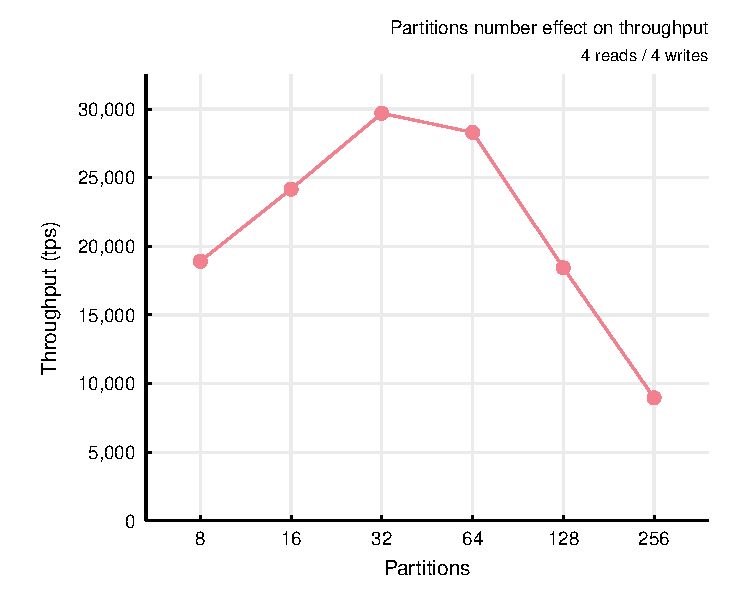
\includegraphics[width=0.5\textwidth]{figures/psi_partitions_throughput.pdf}
\vspace{-0.75cm}
\end{center}
\caption{Performance degradation of fastPSI as the number of partitions increases.}
\label{fig:fastpsi_partition_throughput}
\end{figure}

   \cleardoublepage
\chapter{Related Work}
\label{chapter:related_work}

In this chapter we give an overview of the previous work in the settings of transactional protocols, consistency, and application robustness. We also highlight the main differences between our contributions and previous approaches.

% For robustness: Fekete for first establishing the concept, and Gotsman for showing how
% robustness can be applied to PSI

\paragraph{Application Robustness.} The notion of robustness as applied to databases was first investigated by Fekete et al.~\citep{fekete_ssi}, proposing a way to analyse if applications were robust against Snapshot Isolation (SI)~\citep{sql-critique}. The work of Fekete et al. has resulted in the proliferation of static analysis tools for detecting the presence of anomalies in applications~\citep{sudhir_static}, as well as several run-time techniques for ensuring serialisable transactions~\citep{ports_postgres}. More recently, Bernardi and Gotsman~\citep{concur_robustness} proposed several robustness criteria for a variety of consistency models, including Parallel Snapshot Isolation (PSI)~\citep{psi-intro}. Our work on fastPSI builds on the robustness criteria of Parallel Snapshot Isolation and of Snapshot Isolation to build a hybrid protocol that allows programmers to selectively strengthen consistency guarantees for individual transactions.

% For entity groups: Megastore provided ACID transactions inside an entity group, and a relaxed
% consistency model across groups.

\paragraph{Entity Groups.} The concept of \emph{entity} was introduced by Helland~\citep{helland_entity} to refer to a self-contained data object, with application-defined boundaries, and uniquely identified by an entity key. In addition, Helland argued for the entity to be the largest \emph{scope of transactional serialisability}: transactions can only guarantee atomicity for objects held within the same entity, and are prevented from modifying objects across entities.

Later systems, such as Megastore~\citep{baker_megastore}, introduced the concept of \emph{entity groups}, disjoint aggregations of individual entities, allowing transactions to access distinct entities. Such systems offered strong consistency for transactions accessing entities within a group, while offering almost no consistency guarantees for transactions that accessed different entity groups. Such systems broadened the scope of transactional serialisability to encompass entire entity groups. In contrast, fastPSI provides PSI for all transactions, even those that access objects in multiple entity groups. At the same time, it further strengthens the consistency guarantees for transactions accessing only individual entity groups, by providing SI.

\paragraph{Strong Consistency Protocols.} Although there is a large variety of protocols providing strong consistency, here we focus on those that provide similar guarantees to those in fastPSI, as well as others from which we draw inspiration in the design of our protocol.

% For PSI: Walter paper, used vector timestamps (similar to VCs), but fixed at the beginning of transactions, hence has base freshness. Partial replication, syncs in the background to achieve monotonic timestamps.

Walter, designed by Sovran et al.~\citep{psi-intro}, is a transactional key-value store that offers Parallel Snapshot Isolation. To track causality relations between transactions, Walter uses vector timestamps, similar to the version vectors we use in fastPSI. In contrast with our approach, Walter can only offer snapshots with base freshness, as transactions fix a start timestamp at the beginning of their execution. As a result, the system may experience a higher rate of aborted transactions due to stale reads. Walter also offers partial replication, but the combination of replication and the choice of monotonic start timestamp leads the system to perform global communication in the background with all replicas.

% For NMSI: Ardekani, dependence vectors. First version has one entry per key. Big overhead, but snapshots are always as fresh as possible. Partitioned dependence vectors have less overhead, at the cost of only achieving forward freshness. (Genuine) Partial replication, atomic multicast.

Proposed by Saeida Ardekani et al.~\citep{ardekani_nmsi}, Jessy is a similar transactional key-value store, and the first system to provide Non-Monotonic Snapshot Isolation (NMSI). Unlike Walter, however, transactions in Jessy observe forward freshness in their snapshots, allowing greater scalability. To support consistent snapshots, Jessy uses a data structure called dependence vector, also similar to a version vector, with a number of entries either equal to the number of objects, or equal to the number of partitions. The former approach suffers from a big overhead, although it allows transactions to read versions of objects as fresh as possible. With one entry per partition, Jessy offers greater scalability, at the cost of introducing spurious conflicts between transactions. In fastPSI, we follow a similar approach, using version vectors with one entry per partition. Like Walter, Jessy also supports partial replication. However, Jessy relies on atomic multicast primitives~\citep{guerraoui_multicast}, instead of the two-phase commit protocol used in Walter and in our own protocol, fastPSI.

Another protocol that provides NMSI is Blotter, proposed by Moniz et al.~\citep{moniz_blotter}. In contrast with Jessy, Blotter supports full replication through the use of Paxos commit~\citep{gray_paxos_commit}. The design of Blotter shows how the properties of NMSI, like forward freshness, can be used to design protocols with full replication without loss of scalability.

Peluso et al.~\citep{peluso_gmu} proposed GMU, a transactional protocol that uses vector clocks to track causal dependencies. Much of the design of fastPSI is inspired by GMU, including its clock mechanism, as well as the approaches to build causally consistent snapshots. The consistency guarantees are different, however, as transactions in GMU satisfy the \emph{Extended Update Serialisability} (EUS)~\citep{hansdah_update_ser, adya_thesis} consistency model. EUS guarantees serialisability for update transactions, while read-only transactions can observe different commit orders for non-conflicting transactions, similar to the guarantees offered by the causally compatible snapshots of fastPSI. Even though GMU offers a stronger consistency model than our protocol, GMU always commits read-only transactions, in contrast with the possibility of aborts under fastPSI when transactions cannot satisfy SI and PSI for the same snapshot.

   \cleardoublepage
\chapter{Conclusion}
\label{chapter:conclusion}

\todo{
Talk about the limitations of our approach, coarse grained dependency tracking. Solution: large number of partitions.

Say again what we introduced (a consistency model, a protocol an its implementation, an evaluation), and what we took out of it -> read aborts? performance related to RC and SER.
}

   \appendix
   \cleardoublepage
\chapter{Serialisable and Read Committed Protocols}
\label{appendix:code}

In this appendix we give a quick overview of the protocols we implemented to compare against the fastPSI implementation. For simplicity, both protocols are minor modifications of the original one, although the implementations are still efficient. For each protocol, we summarise the most relevant changes with respect to fastPSI, and give the full pseudocode. The implementation for both protocols is freely available on GitHub~\citep{fastPSIclient, pvc-server}.

\section{Serialisability}
\label{appendix:ser}

Recall from~\ref{sect:ser} that under serialisability transactions appear to execute one after the other. However, it does not guarantee a real-time order among them: an implementation is free to reorder the commit order of transactions as long as the resulting execution still satisfies serialisability. Since our original protocol guarantees Parallel Snapshot Isolation, it is sufficient to prevent the write skew and the long fork anomalies. To do so, we expand fastPSI with several changes. A summary of the state of a server is reflected in Figure~\ref{fig:ser-prot-ds-table}, and the pseudocode of the protocol can be found in Figures~\ref{fig:ser_init}--\ref{fig:ser_termination}.

\paragraph{Track versions of read objects.} Read-only transactions need to observe consistent data that it's not too stale, or overwritten by concurrent transactions. In order to enforce this guarantee, we add a new piece of information to the transaction context: the \emph{read-set} of a transaction keeps track of the objects that it reads, along with the commit time of the version of the object read. When a client receives a $\READRETURN$ message after issuing a read of an object $x$ on behalf of a transaction $\tx$, it incorporates the commit time of $x$ in $\tx$'s read-set, $\tx.\RS$ (line~\ref{alg:ser_rs_update}). It suffices to store the $j$-th entry of $x$'s \emph{commit vector}, that is, the \emph{sequence number} assigned to the transaction that wrote the version of $x$ read by $\tx$. The read-set of a transaction is initialised to the empty set (line~\ref{alg:ser_start_tx}) when the transaction starts.

\paragraph{Avoid stale reads.} Recall from Section~\ref{sect:psi} that the long fork anomaly occurs whenever concurrent transactions are able to observe different orderings of non-conflicting transactions. Such anomaly can be precluded by forcing transactions to observe the latest version of an object. The protocol enforces this property during the validation of a transaction $T$. When a transaction $T$ prepares to commit, it performs a two-phase commit among the servers storing the objects read and written by the transaction (lines~\ref{alg:ser_send_prepare}--\ref{alg:ser_send_prepare_2}). Upon receiving a $\PREPARE$ message, a server $s_i$ checks that, for the objects that $\tx$ read, the version of those objects is the most up-to-date in the database of $s_i$ (line~\ref{alg:ser_conflict_check}, last condition). It does so by comparing the version of the object stored in the transaction's read-set ($\localRS$) against the latest version as reflected by the $\VersionLog$ of the object ($\VersionLog[x].\last.\Vcomm$). The server also needs to perform the check against concurrently-committing transactions (line~\ref{alg:ser_conflict_check}, first condition): a server checks that the read-set of a transaction $\tx$ does not overlap with the write-set of any other concurrently-committing transaction, thereby making $\tx$'s read stale. If the version that $\tx$ read is stale, the server $s_i$ votes $\abort$ (line~\ref{alg:ser_vote_abort}). Since we assume that transactions read an object before writing to it (and thus, $\tx.\WS \subseteq \tx.\RS$) the stale read check also precludes stale writes.

\paragraph{Avoid read-write conflicts.} We can preclude the write skew anomaly, introduced in Section~\ref{sect:si}, by forcing transactions to observe the writes of concurrent transactions as soon as those updates are reflected in the state of the database. A history that exhibits a write skew, such as $h = r_1(x_0).r_1(y_0).r_2(x_0).r_2(y_0).w_1(x_1).w_2(y_2).c_1.c_2$, can only be serialisable by aborting either $\tx_1$ or $\tx_2$. In the protocol, this is avoided by precluding \emph{read-write} conflicts: in the previous history, $\tx_2$ \emph{overwrites} the version of $y$ that $\tx_1$ read. Also, $\tx_1$ overwrites the version of $x$ that $\tx_2$ reads, which is also considered a read-write conflict. Both kinds of conflict can be precluded during the validation of a transaction (line~\ref{alg:ser_conflict_check}, first condition): a server checks that the write-set of a transaction $\tx$ does not overlap with the read-set of any other concurrently-committing transaction (thereby invalidating the read of such concurrent transaction). If any of the checks is true, the server votes $\abort$ (line~\ref{alg:ser_vote_abort}).

\begin{figure}[htb!]
\noindent\adjustbox{max width=\paperwidth}{\footnotesize
\begin{tabularx}{\linewidth}{|c|p{7cm}|X|}
  \hline
  \multicolumn{3}{|c|}{\textbf{Variables at a server $s_i$}} \\
  \hline
  \textbf{Name} & \textbf{Domain} & \textbf{Description} \\
  \hline
  $\lastprep$ & {\sf Integer} & The number of update transactions that tried to
  commit at the server.
\\
  \hline
  $\VersionLog$ & ${\sf Map}[\keytype,$ ${\sf
    Set}[\langle \valuetype\ \val, \vctype\ \Vcomm\rangle]]$ & Database:
  a mapping from objects to lists of pairs of a value and the
  commit vector of the transaction that wrote it. The lists are ordered
  by the $i$-th component of the commit vectors.
\\
  \hline
  $\CommitLog$
  & ${\sf Sequence}[\langle\transtype\ T,$ $\vctype\ \Vaggr \rangle]$
  & Log of update transactions $T$ committed at the server, ordered by
  $\Vaggr[i]$. Here $\Vaggr$ is the aggregate vector of $T$: the join of the
  commit vectors of all transactions up to $T$ in $\CommitLog$.
\\
  \hline
  $\LocalTime$ & $\vctype$ & The join of the commit vectors of all
  transactions in $\CommitLog$.
\\
  \hline
  $\CommitQueue$

  & Sequence$[\langle \transtype, {\sf State}, {\sf ReadSet}, {\sf WriteSet} \rangle]$ where ${\sf State}=\{\pending,\ready\}$

  & Queue containing information about update transactions trying to commit at the server.
\\
  \hline
  \hline
  \multicolumn{3}{|c|}{\textbf{Context for a transaction $T$ at a client $c_i$}} \\
  \hline
  $T.\RS$ & ${\sf ReadSet}$ & Read-set of $T$.
\\
  \hline
  $T.\WS$ & ${\sf WriteSet}$ & Write-set of $T$.
\\
  \hline
  $T.\hasRead$ & ${\sf Vector}[{\sf Bool}]$ & Mapping showing whether $T$ has
  read a given partition.
\\
  \hline
  $T.\VCaggr$ & $\vctype$ & Snapshot vector: determines snapshots fixed at
  partitions $T$ has read from and possible causal dependencies at all other
  partitions.
\\
  \hline
  $T.\VCdep$ & $\vctype$ & Dependency vector, representing all causal
  dependencies developed by $T$ during its execution.
\\
  \hline
\end{tabularx}
}
\caption{List of variables used in the Serialisable protocol, where ${\sf ReadSet} = {\sf Set}[\langle \keytype, {\sf Integer}\rangle]$ and ${\sf WriteSet} = {\sf Set}[\langle \keytype, \valuetype \rangle]$}
\label{fig:ser-prot-ds-table}
\end{figure}

\begin{figure}[h]
\begin{algorithm}[H]
  \setcounter{AlgoLine}{0}
  % Start
  \SubAlgo{\Fun ${\tt start}()$}{
    \Return{$\KwSty{new}\ \transtype(
      \WS= \emptyset,
      \RS= \emptyset,
      \hasRead = \vec{\bot},
      \VCaggr = \vec{0},
      \VCdep = \vec{0})$
    };\label{alg:ser_start_tx}
  }

  \smallskip

  % Write
  \SubAlgo{\Fun ${\tt write}(T, x, v)$}{
    $\tx.\WS \leftarrow \left(\tx.\WS\ \backslash\ \{\langle x, \_ \rangle\}\right) \cup \{\langle x,v\rangle\}$\;
  }
\end{algorithm}
\caption{Initialisation of a transaction and update of an object \emph{x} at client $c_i$ under serialisability.}
\label{fig:ser_init}
\end{figure}

\begin{figure}[h]
\begin{algorithm}[H]
  % Read
  \SubAlgo{\Fun ${\tt read}(T, x)$}{
    \If{$\langle x, v \rangle \in \tx.\WS$}{
      \Return{$v$}\;
    }

    $j \leftarrow \partitionof(x)$\;
    \Send{$\READREQUEST(x, T.\VCaggr, T.\hasRead)$} \KwTo $s_j$\;
    \Receive{$\READRETURN(m)$} \KwFrom $s_j$\;
    \uIf{$m = \abort$} {
      \Throw{$\abort$}\;
    }
    \ElseIf{$m = \langle v,\localVdep,\localVaggr \rangle$}{
      $\tx.\hasRead[j] \leftarrow \true$\;
      $\tx.\RS \leftarrow
        \left(\tx.\RS\ \backslash\ \{\langle x, \_ \rangle\}\right)
        \cup
        \{\langle x, \localVdep[j] \rangle\}$\;\label{alg:ser_rs_update}
      $\tx.\VCdep \leftarrow \max(\tx.\VCdep,\localVdep)$\;
      $\tx.\VCaggr \leftarrow \max(\tx.\VCaggr,\localVaggr)$\;
      \Return{$v$}\;
    }
  }

  \smallskip

  % ReadRequest
  \SubAlgo{\WhenReceived $\READREQUEST(x, \argVCaggr, \argHasRead)$ \KwFrom $c_j$}{
    \uIf{$\argHasRead[i]$} {
      $V \leftarrow \argVCaggr$\;
    }
    \Else{
      \Until{$\mrvc[i] \ge \argVCaggr[i]$}\;
      $r \leftarrow \max\{r \in \CommitLog \mid \forall j.\, \argHasRead[j] {\implies} \left(r.\Vaggr[j] \le \argVCaggr[j]\right)\}$\;
      \If{$r.\Vaggr[i] < \argVCaggr[i]$}{
        \Send{$\READRETURN(\abort)$} \KwTo $c_j$\;
        \Return\;
      }
      $V \leftarrow r.\Vaggr$\;
    }
    $\ver = \max\{\ver \in \VersionLog \mid ver.\Vcomm[i] \le V[i]\}$\;
    \Send{$\READRETURN(\ver.\val, \ver.\Vcomm,V)$} \KwTo $c_j$\;
  }
\end{algorithm}
\caption{Serialisable local and remote read of object \emph{x}}
\end{figure}

\begin{figure}[h]
\begin{algorithm}[H]
  % Commit
  \SubAlgo{\Fun ${\tt commit}(T)$\label{alg:ser_commit_start}}{
    \ForAll{$\partj \in \partitions(\tx.\RS \cup \tx.\WS)$\label{alg:ser_send_prepare}}{
      \Send{$\PREPARE(T, T.\RS, T.\WS, \VCdep)$} \KwTo $\partj$\;\label{alg:ser_send_prepare_2}
    }

    $\commitVC \leftarrow \tx.\VCdep$\;
    $\outcome \leftarrow \commit$\;

    \ForAll{$\partj \in \partitions(\tx.\RS \cup \tx.\WS)$}{
      \Receive{$\VOTE(m)$} \KwFrom $\partj$\;
      \uIf{$m = \langle T, \abort \rangle$}{
        $\outcome \leftarrow \abort$\;
        \Break\;
      }
      \ElseIf{$m = \langle T, \commit, k \rangle$}{
        $\commitVC[j] \leftarrow k$\;
      }
    }

    \ForAll{$\partj \in \partitions(\tx.\RS \cup \tx.\WS)$}{
      \Send{$\DECIDE(\tx, \commitVC,\outcome)$} \KwTo $\partj$\;
    }

    \Return{$\outcome$}\;
  }

  \smallskip

  % Prepare
  \SubAlgo{\WhenReceived $\PREPARE(T, \localRS, \localWS, \localVdep)$ \KwFrom $c_j$}{
    \If{$
      (\exists T'.\ (\langle T', \pending, \localRS', \localWS' \rangle \in \cqueue$
      \begin{tabularx}{\linewidth}{l}
        \quad\quad\quad$\vee\ \langle T', \ready, \_, \_, \_ \rangle \in \cqueue)$\\
        \quad\quad\quad$\wedge\
        (\localWS' \cap \localRS \ne \emptyset
          \wedge \localRS' \cap \localWS \ne \emptyset)$\\
        $\vee \left(
          \exists x. \ \langle x, vsn \rangle \in \localRS
          \wedge (\VersionLog[x].\last.\Vcomm[i] > vsn)\right)$\\
      \end{tabularx}\label{alg:ser_conflict_check}
    }{
      \Send{$\VOTE(t, \abort)$} \KwTo $c_j$\;\label{alg:ser_vote_abort}
      \Return\;
    }

    $\lastprep \leftarrow \lastprep + 1$\;
    $\cqput(\tx, \pending, \localRS, \localWS)$\;
    \Send{$\VOTE(\tx, \commit, \lastprep)$} \KwTo $c_j$\;
  }

  \smallskip

  % Decide
  \SubAlgo{\WhenReceived $\DECIDE(T, \commitVC, \outcome)$ \KwFrom $c_j$}{
    \uIf{$\outcome = \commit$}{
      $\cqupdate(\langle \tx, \ready, \_, \_, \commitVC\rangle)$\;
    }
    \Else{
      $\cqremove(\tx)$\;
    }
  }

  \smallskip

  % Queue head
  \SubAlgo{\Upon $\langle T, \ready, \_, \localWS, \commitVC\rangle = \cqhead()$}{
    \ForAll{$\{\langle x , v \rangle \mid \langle x , v \rangle \in \localWS \wedge \partitionof(x) = i\}$} {
        $\vlapply(\langle x , v , \commitVC \rangle)$\;
    }

    $\mrvc \leftarrow \max(\mrvc,\commitVC)$\;
    $\cladd(T, \mrvc)$\;
    $\cqremove(T)$\;
  }
\end{algorithm}
\caption{Serialisable termination protocol.}
\label{fig:ser_termination}
\end{figure}

\clearpage

\section{Read Committed}
\label{appendix:rc}

Read Committed (RC) is the weakest consistency model that satisfies the \emph{isolation} property required by ACID transactions. It forbids concurrent transactions from observing any data that has not been committed, but it does not place any restriction on the ordering of transactions, and does not preclude write-write conflicts. Thus, transactions may be ordered in any way. Figure~\ref{fig:rc-prot-ds-table} shows a summary of the data structures involved in the protocol.

\begin{figure}[h]
\noindent\adjustbox{max width=\paperwidth}{\footnotesize
\begin{tabularx}{\linewidth}{|c|p{5.5cm}|X|}
  \hline
  \multicolumn{3}{|c|}{\textbf{Variables at a server $s_i$}} \\
  \hline
  \textbf{Name} & \textbf{Domain} & \textbf{Description} \\
  \hline
  $\CommitQueue$

  & Sequence$[\langle \transtype, {\sf State}, {\sf WriteSet} \rangle]$ where ${\sf State}=\{\pending,\ready\}$

  & Queue containing information about update transactions trying to commit at the server. \\
  \hline
  Database

  & Set$[\langle {\sf Object} ,{\sf Value}\rangle]$

  & Set representing the key-value store as a mapping from objects to values. \\
  \hline\hline
  \multicolumn{3}{|c|}{\textbf{Context for a transaction $T$ at a client $c_i$}} \\
  \hline
  $T.\WS$ & ${\sf WriteSet}$ & Write-set of $T$. \\
  \hline
\end{tabularx}
}
\caption{List of variables used in the Read Committed protocol, where ${\sf WriteSet} = {\sf Set}[\langle \keytype, \valuetype \rangle]$.}
\label{fig:rc-prot-ds-table}
\end{figure}

Since transactions only need to observe the last committed version of an object, it is sufficient to store only one version. Thus, we can substitute the $\VersionLog$ mapping with a \emph{Database}, that simply maps an object to its latest version. In addition, transactions don't need to observe a consistent snapshot of the state of a partition, and therefore we can remove all data structures related to computing a snapshot. This is reflected in the execution of a transaction, as can be seen in Figure~\ref{fig:rc_tx_exection}. A server $s_i$ executing a remote read on behalf of a transaction $\tx$ simply fetches the currently available value of the requested object, and returns it to the client (line~\ref{alg:rc_db_get}).

A protocol satisfying Read Committed still needs to offer atomic visibility. To do so, our implementation uses two-phase commit, guaranteeing that a transaction commits at every partition (line~\ref{alg:rc_commit_start}). Servers that participate during the commit phase always vote $\commit$ (line~\ref{alg:rc_send_vote}), since RC does not preclude write-write conflicts. After a successful commit phase, all servers incorporate the updates of the transaction to its partition state (line~\ref{alg:rc_kv_apply}).

\begin{figure}[h]
\begin{algorithm}[H]
  \setcounter{AlgoLine}{0}
  %  Start
  \SubAlgo{\Fun ${\tt start}()$}{
    \Return{$\KwSty{new}\ \transtype(\WS= \emptyset)$};
  }

  \smallskip

  % Write
  \SubAlgo{\Fun ${\tt write}(T, x, v)$}{
    $\tx.\WS \leftarrow \left(\tx.\WS\ \backslash\ \{\langle x, \_ \rangle\}\right) \cup \{\langle x, v \rangle\}$\;
  }
\end{algorithm}
\caption{Initialisation of a transaction and update of an object \emph{x} at client $c_i$ under Read Committed.}
\end{figure}

\begin{figure}[t]
\begin{algorithm}[H]

  % Read
  \SubAlgo{\Fun ${\tt read}(T, x)$}{
    \If{$\langle x, v \rangle \in \tx.\WS$}{
      \Return{$v$}\;
    }

    $j \leftarrow \partitionof(x)$\;
    \Send{$\READREQUEST(x)$} \KwTo $s_j$\;
    \Receive{$\READRETURN(v)$} \KwFrom $s_j$\;
    \Return{$v$}\;
  }

  \smallskip

  % ReadRequest
  \SubAlgo{\WhenReceived $\READREQUEST(x)$ \KwFrom $c_j$}{
    \Send{$\READRETURN(\kvget(x))$} \KwTo $c_j$\;\label{alg:rc_db_get}
  }

  \smallskip

    % Commit
  \SubAlgo{\Fun ${\tt commit}(T)$\label{alg:rc_commit_start}}{
    \If{$\ws = \emptyset$}{
      \Return{$\commit$}\;
    }

    \ForAll{$\partj \in \partitions(\tx.\WS)$}{
      \Send{$\PREPARE(T)$} \KwTo $\partj$\;
    }

    $\outcome \leftarrow \commit$\;
    \ForAll{$\partj \in \partitions(\tx.\WS)$}{
      \Receive{$\VOTE(m)$} \KwFrom $\partj$\;
      \If{$m = \langle T, \abort\rangle$}{
        $\outcome \leftarrow \abort$\;
        \Break\;
      }
    }

    \ForAll{$\partj \in \partitions(\tx.\WS)$}{
      \Send{$\DECIDE(\tx, \outcome)$} \KwTo $\partj$\;
    }

    \Return{$\outcome$}\;
  }

    % Prepare
  \SubAlgo{\WhenReceived $\PREPARE(T)$ \KwFrom $c_j$}{
    $\cqput(T, \pending, \WS)$\;
    \Send{$\VOTE(T, \commit)$} \KwTo $c_j$\;\label{alg:rc_send_vote}
  }

  % Decide
  \SubAlgo{\WhenReceived $\DECIDE(T, \outcome)$ \KwFrom $c_j$}{
    \uIf{$\outcome = \commit$}{
      $\cqupdate(\langle T, \ready, \_ \rangle)$\;
    }
    \Else{
      $\cqremove(T)$\;
    }
  }

  \smallskip

  % Queue head
  \SubAlgo{\Upon $\langle T, \ready, \localWS\rangle = \cqhead()$}{
    \ForAll{$\{\langle x, v\rangle \mid \langle x, v \rangle \in \localWS \wedge \partitionof(x) = i\}$}{
      $\kvapply(x, v)$\;\label{alg:rc_kv_apply}
    }
  $\cqremove(T)$\;
  }
\end{algorithm}
\caption{Read Committed execution protocol.}
\label{fig:rc_tx_exection}
\end{figure}


% +--------------------------------------------------------------------+
% | This template uses the BibTeX program to format references.  The
% | 3 lines below create a separate Bibliography section and add
% | an entry for "Bibliography" to the Table of Contents.  The actual
% | data for your references (author, title, journal, date, etc.) are
% | entered in the references.bib file.  See that file for information
% | on how to enter references.
% +--------------------------------------------------------------------+

\bibdata{references}
\bibliographystyle{plainnat}
\bibliography{references}
\addcontentsline{toc}{chapter}{Bibliography}

\end{document}
